

\documentclass[11pt]{article}

\title{ Advancing predictive physical modeling through focused development of model systems to drive new modeling innovations}

\usepackage[top=0.5in, bottom=0.5in, left=0.5in, right=0.5in]{geometry}
\usepackage{helvet}
\usepackage{url} % hypderref?
\usepackage{graphicx}
\graphicspath{{figures/}} % The figures are in a figures/ subdirectory.
\renewcommand{\familydefault}{\sfdefault}
\pagestyle{empty}
%\pagestyle{plain}

% Fancy page-width tables
\usepackage{tabularx}

% Use a package for framed boxes
\usepackage{mdframed}

\usepackage[T1]{fontenc}
\usepackage{amssymb}


\usepackage{setspace}
\usepackage{microtype}

\usepackage{amsfonts}
\usepackage{amsmath}

\usepackage{floatrow}

\usepackage[normalem]{ulem} % for nci.bst

\usepackage{sidecap}
\usepackage[abs]{overpic}
\usepackage{wrapfig}


\usepackage{hyperref}
\hypersetup{colorlinks=true, urlcolor=black, citecolor=black, linkcolor=black}

\usepackage[numbers,sort&compress]{natbib} %comment on first run?

\usepackage{multibib}
%\newcites{full,sampl}{A,B}
\newcites{sampl}{Full List of SAMPL References}
%\newbibliography{full}

%\usepackage[round,authoryear]{natbib}
%\usepackage{cite}
%\setlength{\bibsep}{0.00in}


\newcommand{\doi}[1]{\href{http://dx.doi.org/#1}{doi:#1}}

\newcommand{\ac}[1]{{\sc \lowercase{#1}}}

\renewcommand{\baselinestretch}{.93}
%\renewcommand{\baselinestretch}{.90}
\usepackage{wrapfig} 

\usepackage{bibspacing}
\setlength{\bibspacing}{\baselineskip}




\graphicspath{{figs/}}

\makeatletter

\newcommand{\captionfonts}{\footnotesize}

\makeatletter  % Allow the use of @ in command names
\long\def\@makecaption#1#2{%
  \vskip\abovecaptionskip
  \sbox\@tempboxa{{\captionfonts #1: #2}}%
  \ifdim \wd\@tempboxa >\hsize
    {\captionfonts #1. #2\par}
  \else
    \hbox to\hsize{\hfil\box\@tempboxa\hfil}%
  \fi
  \vskip\belowcaptionskip}      
\makeatother

\renewcommand{\figurename}{{\bf Figure}}

% Page numbering.
%\pagestyle{plain}
%\pagenumbering{arabic}

\setlength{\abovecaptionskip}{-5pt}

\makeatother

\renewcommand{\refname}{Bibliography and References Cited}

\setlength{\parindent}{0pt} % Don't indent first line
%\setlength{\parskip}{1ex plus 0.5ex minus 0.2ex} % Add some space between paragraphs
\setlength{\parskip}{0.8ex} % Add some space between paragraphs

\begin{document}

%======================================
% CITE SAMPL REFS FIRST FOR BETTER COMPRESSION
\phantom{
\citesampl{monroe_converging_2014_sampl,muddana_blind_2014_sampl,gallicchio_bedam_2015-1_sampl,mikulskis_free-energy_2014_sampl,hsiao_prediction_2014_sampl,bhakat_resolving_2016_sampl,pal_combined_2016_sampl,yin_sampl5_2016_sampl,bosisio_blinded_2016_sampl,tofoleanu_absolute_2016_sampl,mobley_blind_2014-1_sampl,muddana_sampl4_2014_sampl,sullivan_binding_2016_sampl,deng_distinguishing_2015_sampl,li_testing_2014_sampl,paranahewage_predicting_2016_sampl,klamt_prediction_2016_sampl,tielker_sampl5_2016_sampl,konig_calculating_2016_sampl,luchko_sampl5:_2016_sampl,santos-martins_calculation_2016_sampl,perryman_virtual_2014_sampl,konig_predicting_2014_sampl,voet_combining_2014_sampl,park_extended_2014_sampl,rustenburg_measuring_2016_sampl,reinisch_prediction_2014_sampl,muddana_sampl4_2014-1_sampl,manzoni_prediction_2014_sampl,sandberg_predicting_2014_sampl,brini_adapting_2016_sampl,kamath_prediction_2016_sampl,diaz-rodriguez_predicting_2016_sampl,kenney_prediction_2016_sampl,caldararu_binding_2016_sampl,genheden_all-atom/coarse-grained_2016_sampl,chung_extended_2016_sampl,koziara_testing_2014_sampl,yin_overview_2016_sampl,Bannan:2016:JComputAidedMolDes_sampl,Lee:2016:JComputAidedMolDes_sampl,Jones:2016:JComputAidedMolDes_sampl,Pickard:2016:JComputAidedMolDes_sampl, cao_absolute_2014_sampl,muddana_prediction_2012_sampl,gibb_binding_2013_sampl,klimovich_predicting_2010_sampl,mobley_alchemical_2012_sampl,muddana_sampl3_2012_sampl,skillman_sampl3_2012_sampl,Newman:2011:JComputAidedMolDes_sampl,gallicchio_virtual_2014_sampl,klamt_blind_2010_sampl,fennell_modeling_2011_sampl,ellingson_analysis_2010_sampl,surpateanu_evaluation_2011_sampl,purisima_rapid_2010_sampl,konig_predicting_2011_sampl,kehoe_testing_2011_sampl,kumar_computational_2012_sampl,meunier_predictions_2010_sampl,genheden_extensive_2014_sampl,beckstein_prediction_2014_sampl,coleman_sampl4_2014_sampl,hogues_exhaustive_2014_sampl,reinisch_prediction_2012_sampl,kulp_fragment-based_2012_sampl,klamt_conclusions_2010_sampl,fu_fast_2014_sampl,hamaguchi_force-field_2012_sampl,colas_virtual_2014_sampl,ellingson_efficient_2014_sampl,sulea_predicting_2011_sampl,geballe_sampl2_2010_sampl,ribeiro_prediction_2010_sampl,skillman_sampl2_2010_sampl,gallicchio_prediction_2012_sampl,mikulskis_binding_2011_sampl,geballe_sampl3_2012_sampl,guthrie_sampl4_2014_sampl,nicholls_sampl2_2010_sampl,soteras_performance_2010_sampl,lawrenz_thermodynamic_2012_sampl,sulea_exhaustive_2011_sampl,beckstein_prediction_2011_sampl,benson_prediction_2012_sampl,kast_prediction_2010_sampl,mobley_predictions_2009_sampl,newman_practical_2009_sampl,klamt_prediction_2009_sampl,guthrie_blind_2009_sampl,marenich_performance_2009_sampl,sulea_prediction_2009_sampl,nicholls_samp1_2009_sampl,nicholls_predicting_2008_sampl,chamberlin_performance_2008_sampl,Gosink:2017:J.Phys.Chem.B_sampl, Yang:2017:arXiv:1705.10035[q-bio]_sampl, shirts_lessons_2016_sampl, Bansal:2017:JComputAidedMolDes_sampl}
\cite{Moult:2014:Proteins, Monastyrskyy:2016:Proteins, Moult:2016:Proteins, Prill:2011:Sci.Signal., Eisenstein:2013:NatBiotech, Saez-Rodriguez:2016:NatRevGenet, Bell:2010:CHANCE, ::XPRIZE, Kay:2011:R&DManage, XPrize:2017:Wikipedia, Mobley:2017:eScholarship, Gathiaka:2016:JComputAidedMolDes}
}

%%%%%%%%%%%%%%%%%%%%%%%%%%%%%%%%%%%%%%%%%%%%%%%%%%%%%%%%%%%%%%%%%%%%%%%%%%%
% SPECIFIC AIMS
%%%%%%%%%%%%%%%%%%%%%%%%%%%%%%%%%%%%%%%%%%%%%%%%%%%%%%%%%%%%%%%%%%%%%%%%%%%

%{\large \bf SPECIFIC AIMS}

%\eject

%%%%%%%%%%%%%%%%%%%%%%%%%%%%%%%%%%%%%%%%%%%%%%%%%%%%%%%%%%%%%%%%%%%%%%%%%%%
% SIGNIFICANCE
%%%%%%%%%%%%%%%%%%%%%%%%%%%%%%%%%%%%%%%%%%%%%%%%%%%%%%%%%%%%%%%%%%%%%%%%%%%

{\Large \bf SIGNIFICANCE}


\textbf{Physical modeling is poised to transform drug discovery and chemical biology by enabling true molecular design.}
While modeling is used extensively in drug discovery, it mainly assists in idea generation and filtering large libraries of compounds for screening. 
Instead, we envision using computational techniques extensively to guide design. 
Consider a medicinal chemist in the not-too-distant future who has just received potency data for newly-synthesized inhibitors against a desired biomolecular target. 
Before leaving work, she generates ideas for perhaps 100 new compounds for synthesis, setting her computer to work overnight. 
By morning, the idea compounds have been prioritized based on reliable predictions of their affinity for the desired target, selectivity against antitargets, solubility, and membrane permeability.  
Looking through the top few compounds, she selects some for synthesis. 
If synthesizing and testing each compound takes several days, this workflow could compress roughly a year's work into a few days.

While not yet a reality, significant strides have been made toward accurate binding affinities~\cite{mobley_perspective_2012, christ_accuracy_2014, deng_distinguishing_2015, Sherborne:2016:JComputAidedMolDes, schrodinger_accurate_2015, christ_binding_2016, cui_affinity_2016, verras_free_2016, Aldeghi:2017:J.Am.Chem.Soc.}, solubilities~\cite{Schnieders:2012:J.Chem.TheoryComput., park_absolute_2014, liu_using_2016}, selectivity and drug resistance~\cite{leonis_contribution_2013, Aldeghi:2017:J.Am.Chem.Soc.}, and membrane permeability~\cite{lee_permeability_2016, comer_permeability_2014}. 
A considerable amount of science and engineering still remains to be done to make this vision a reality, but the question now seems more one of \emph{when} rather than \emph{whether} it is achieved.

Widespread availability of inexpensive graphics processing units (GPUs) provides a 100-fold increase in price-to-performance ratio over CPUs, while advances in automation~\cite{liu_lead_2013} and sampling protocols have helped simulation-based techniques reach the point where they now begin to be genuinely useful in guiding drug discovery for a limited \emph{domain of applicability}~\cite{mikulskis_large-scale_2014, homeyer_binding_2014, Sherborne:2016:JComputAidedMolDes,  schrodinger_accurate_2015, christ_binding_2016, cui_affinity_2016, verras_free_2016}.
Specifically, in some situations, free energy calculations appear to be capable of achieving RMS errors of 1--2 kcal/mol with current force fields, even in prospective applications, sufficient to drastically reduce the number of molecules that must be synthesized and assayed~\cite{shirts_free-energy_2010, Aldeghi:2017:J.Am.Chem.Soc., schrodinger_accurate_2015}.
As a consequence, pharmaceutical companies have rapidly adopted these methods in active discovery projects~\cite{Sherborne:2016:JComputAidedMolDes}.

\textbf{Despite progress, current modeling methods suffer from severe limitations hindering their widespread use in molecular design.}
For example, even ``small'' protein conformational changes not gracefully handled by current methodologies can yield errors up to 5 kcal/mol in calculated binding free energies~\cite{lim_sensitivity_2016}, force field limitations still pose major challenges~\cite{rocklin_blind_2013}, and the inability to treat important chemical effects like protonation and tautomer equilibria drastically limits the domain of applicability.
{\bf For many pharmaceutically relevant systems, the most important sources of error---and modeling challenges---are not yet clear.~\cite{Sherborne:2016:JComputAidedMolDes}}

These hurdles frustrate progress in the field. 
Method developers focus on addressing some specific challenges, but {\bf new methods are tested on disparate datasets making it difficult to gauge progress and identify valuable methods when they are developed}.
And applications projects tend not to take advantage of the latest methods---in part because their utility is not yet clear. 
As a result, valuable methods can languish relatively unused in the literature for many years without impacting applications in drug discovery.

{\bf We propose an iterated Challenge-based approach to drive methodological innovation via crowdsourcing.} 
A series of community blind prediction Challenges will test and push the limits of predictive techniques, providing a bridge between challenging but tractable problems and pharmacologically relevant but currently intractable problems.
Our Statistical Assessment of Modeling of Proteins and Ligands (SAMPL) Challenges take advantage of proven crowdsourcing-based approaches to science (discussed below), allowing head-to-head comparisons of existing methods and fostering development of new methods.
Regular, progressive Challenges provide an environment for rapid innovation from ``unconventional innovators''~\cite{Kay:2011:R&DManage} from diverse fields who form collaborative teams, applying and integrating distinct approaches~\cite{Saez-Rodriguez:2016:NatRevGenet}.

{\bf Meaningful Challenges require new targeted data collection.}
A key focus of this proposal is on generating new data to test methods in prospective Challenges in an unbiased way. 
New data provides additional value over retrospective tests on literature data:
First, we are able to ensure high data quality and ensure we can collect additional data for the same systems as needed
Additionally, retrospective tests do not test predictive power---they easily fall victim to significance hacking or inadvertent overfitting~\cite{Nuzzo:2015:Nature}.
Retrospective work also may utilize prior knowledge, even if unintentionally.  
For example, if a ligand binding mode is already known crystallographically, a researcher may use that binding mode in retrospective tests, whereas prospective or design work requires first selecting among candidate binding modes, introducing substantial uncertainty unaccounted for in the retrospective statistics~\cite{mobley_predicting_2007, boyce_predicting_2009, mobley_perspective_2012}.
While discovery projects provide one opportunity for prospective tests, they are not adequate---partly because often, the predicted compounds are in fact never tested~\cite{christ_binding_2016} or the experimental data necessary to assess prediction quality (binding affinities or crystallography, for example) is absent.

{\bf Tractable Challenges inspire rapid progress, while Challenges that are too difficult accomplish little}~\cite{Saez-Rodriguez:2016:NatRevGenet}. 
We require high quality Challenges carefully designed specifically to maximize community learning by pushing the limits of current technology.
While the Drug Design Data Resource (D3R~\cite{Gathiaka:2016:JComputAidedMolDes}) also fields blind Challenges, these rely on contributed experimental protein-ligand datasets from now-defunct pharmaceutical discovery programs~\cite{Gathiaka:2016:JComputAidedMolDes}. 
D3R Challenges provide a necessary \emph{benchmark} for real-world performance, but provide only modest new insight to drive improvement because a multitude of issues are be responsible for poor performance~\cite{D3R_lessons_learned}.

\textbf{Methodology improvement is most rapid when complex goals are achieved via tractable intermediate milestones} which can be independently assessed using high quality data~\cite{Saez-Rodriguez:2016:NatRevGenet}.
Thus, we focus on using Challenges to drive and evaluate solutions to specific \emph{component} problems that make it difficult to predict biomolecular interactions.
The Challenge format allows the entire community to learn from both failure and success.
Much as \emph{unit testing} is indispensable for identifying software bugs when complex integration tests fail, Challenges like SAMPL are valuable in pinpointing modeling errors, especially when projects like D3R highlight overall performance problems.
Hence, SAMPL Challenges focus on predicting properties that isolate likely sources of error, such as physical properties of small molecules (hydration free energies, aqueous tautomer ratios, partition or distribution coefficients between aqueous and nonpolar phases) or binding in systems of reduced complexity (such as host-guest complexation, or binding of fragments to trypsin and HIV integrase).


%%%%%%%%%%%%%%%%%%%%%%%%%%%%%%%%%%%%%%%%%%%%%%%%%%%%%%%%%%%%%%%%%%%%%%%%%%%%%%%%
%SAMPL HISTORY
\begin{wrapfigure}[24]{r}{7cm}
\vspace{-0.2in}
\begin{centering}
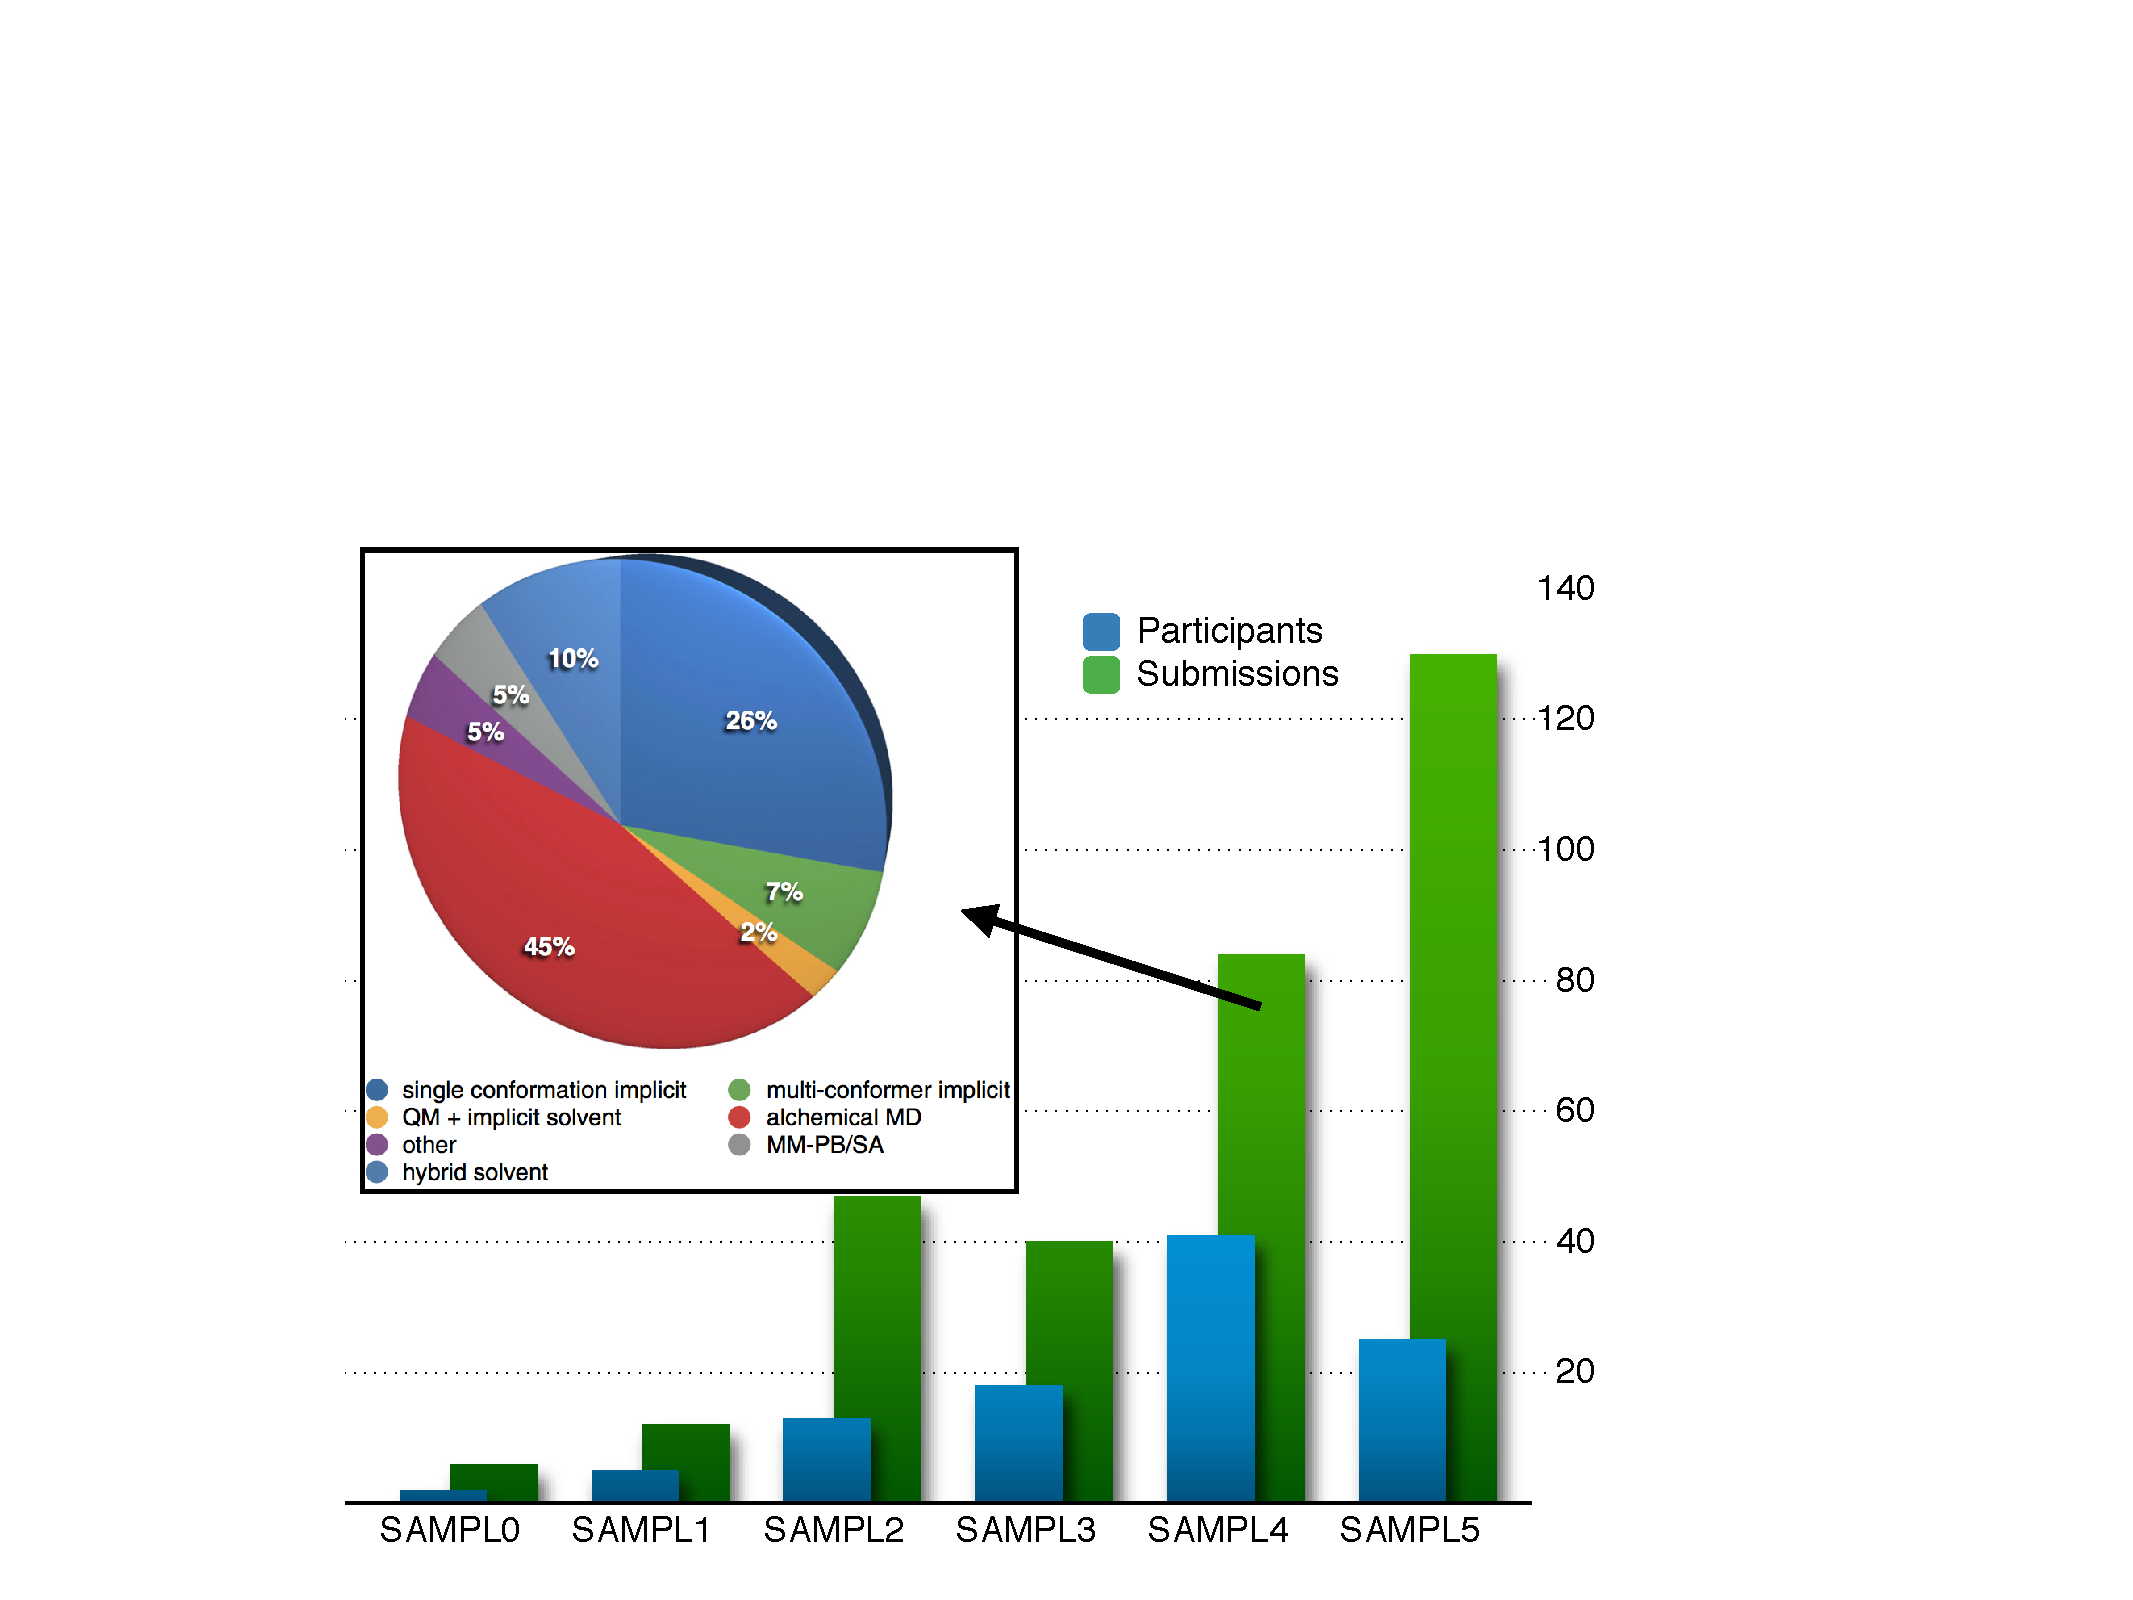
\includegraphics[width=\textwidth]{figures/history_v1.pdf}

\end{centering}
\footnotesize
\caption{\label{figure:sampl_history}  
\textbf{SAMPL historical participation~\cite{mobley_blind_2014-1}.} 
Historical participation in SAMPL host-guest + solvation/distribution Challenges has climbed rapidly, and we expect this trend to continue. The number of participating groups is shown in blue, and the number of submissions in green. The inset shows the diversity of methods employed for the SAMPL4 hydration Challenge, which is typical for SAMPL. 
While SAMPL5 had fewer participants, this was because SAMPL4 included an HIV integrase binding prediction Challenge, whereas D3R handled such data after SAMPL4.
Despite this shift, the number of submissions in SAMPL5 was the highest yet.
}
\end{wrapfigure}
%%%%%%%%%%%%%%%%%%%%%%%%%%%%%%%%%%%%%%%%%%%%%%%%%%%%%%%%%%%%%%%%%%%%%%%%%%%%%%%%

The {\bf SAMPL series of Challenges has already proven it can drive dramatic improvements in modeling methodologies}.
SAMPL, born out of frustration with the lack of venues for comparing predictive accuracy on a level playing field, was initiated by Anthony Nicholls of OpenEye software in 2007/2008~\cite{nicholls_predicting_2008}, and has run Challenges approximately every two years since then~\cite{nicholls_samp1_2009, mobley_predictions_2009, geballe_sampl2_2010, geballe_sampl3_2012, mobley_blind_2014-1, muddana_sampl4_2014, Bannan:2016:JComputAidedMolDes, yin_overview_2016}.
Governance transitioned to an unfunded academic collaboration among the PI and co-Investigators during SAMPL3 in 2012; this collaboration ran SAMPL4 (2014), SAMPL5 (2016), currently SAMPL6 (2017-2018). 
The PI of this proposal (Mobley) was a primary organizer of SAMPL4-6 (2014--present).
{\bf SAMPL has demonstrated its utility as a valuable community resource, resulting in $\sim$100 publications typically cited 5--50 times or more each}~\citesampl{monroe_converging_2014_sampl,muddana_blind_2014_sampl,gallicchio_bedam_2015-1_sampl,mikulskis_free-energy_2014_sampl,hsiao_prediction_2014_sampl,bhakat_resolving_2016_sampl,pal_combined_2016_sampl,yin_sampl5_2016_sampl,bosisio_blinded_2016_sampl,tofoleanu_absolute_2016_sampl,mobley_blind_2014-1_sampl,muddana_sampl4_2014_sampl,sullivan_binding_2016_sampl,deng_distinguishing_2015_sampl,li_testing_2014_sampl,paranahewage_predicting_2016_sampl,klamt_prediction_2016_sampl,tielker_sampl5_2016_sampl,konig_calculating_2016_sampl,luchko_sampl5:_2016_sampl,santos-martins_calculation_2016_sampl,perryman_virtual_2014_sampl,konig_predicting_2014_sampl,voet_combining_2014_sampl,park_extended_2014_sampl,rustenburg_measuring_2016_sampl,reinisch_prediction_2014_sampl,muddana_sampl4_2014-1_sampl,manzoni_prediction_2014_sampl,sandberg_predicting_2014_sampl,brini_adapting_2016_sampl,kamath_prediction_2016_sampl,diaz-rodriguez_predicting_2016_sampl,kenney_prediction_2016_sampl,caldararu_binding_2016_sampl,genheden_all-atom/coarse-grained_2016_sampl,chung_extended_2016_sampl,koziara_testing_2014_sampl,yin_overview_2016_sampl,Bannan:2016:JComputAidedMolDes_sampl,Lee:2016:JComputAidedMolDes_sampl,Jones:2016:JComputAidedMolDes_sampl,Pickard:2016:JComputAidedMolDes_sampl, cao_absolute_2014_sampl,muddana_prediction_2012_sampl,gibb_binding_2013_sampl,klimovich_predicting_2010_sampl,mobley_alchemical_2012_sampl,muddana_sampl3_2012_sampl,skillman_sampl3_2012_sampl,Newman:2011:JComputAidedMolDes_sampl,gallicchio_virtual_2014_sampl,klamt_blind_2010_sampl,fennell_modeling_2011_sampl,ellingson_analysis_2010_sampl,surpateanu_evaluation_2011_sampl,purisima_rapid_2010_sampl,konig_predicting_2011_sampl,kehoe_testing_2011_sampl,kumar_computational_2012_sampl,meunier_predictions_2010_sampl,genheden_extensive_2014_sampl,beckstein_prediction_2014_sampl,coleman_sampl4_2014_sampl,hogues_exhaustive_2014_sampl,reinisch_prediction_2012_sampl,kulp_fragment-based_2012_sampl,klamt_conclusions_2010_sampl,fu_fast_2014_sampl,hamaguchi_force-field_2012_sampl,colas_virtual_2014_sampl,ellingson_efficient_2014_sampl,sulea_predicting_2011_sampl,geballe_sampl2_2010_sampl,ribeiro_prediction_2010_sampl,skillman_sampl2_2010_sampl,gallicchio_prediction_2012_sampl,mikulskis_binding_2011_sampl,geballe_sampl3_2012_sampl,guthrie_sampl4_2014_sampl,nicholls_sampl2_2010_sampl,soteras_performance_2010_sampl,lawrenz_thermodynamic_2012_sampl,sulea_exhaustive_2011_sampl,beckstein_prediction_2011_sampl,benson_prediction_2012_sampl,kast_prediction_2010_sampl, mobley_predictions_2009_sampl,newman_practical_2009_sampl,klamt_prediction_2009_sampl,guthrie_blind_2009_sampl,marenich_performance_2009_sampl,sulea_prediction_2009_sampl,nicholls_samp1_2009_sampl,nicholls_predicting_2008_sampl,chamberlin_performance_2008_sampl, Gosink:2017:J.Phys.Chem.B_sampl, Yang:2017:arXiv:1705.10035[q-bio]_sampl, shirts_lessons_2016_sampl, Bansal:2017:JComputAidedMolDes_sampl}.
SAMPL datasets are so valuable to the community that they foster retrospective tests long after the Challenges end (e.g.~\cite{Yang:2017:arXiv:1705.10035[q-bio], Gosink:2017:J.Phys.Chem.B, Harger::J.Comput.Chem., Bradshaw:2016:J.Chem.TheoryComput.}).

Until now, \textbf{SAMPL has relied on donated data and time}, making it impossible to design Challenges specifically to improve modeling as we propose here. 
Despite these limitations, our recent survey reveals that SAMPL has already had a significant effect on the field; past participants are overwhelmingly enthusiastic about SAMPL and the plans we propose here~\cite{Mobley:2017:eScholarship}.
One of our most frequent requests is for modestly larger datasets, which we propose here. 
Our proposed Challenges bridge the gap between calculations of simple physical properties that isolate force field inaccuracies from slow conformational sampling inherent to protein-ligand systems---such as hydration free energies, which can already be calculated fairly accurately~\cite{mobley_blind_2014-1}---and the D3R Grand Challenges on protein-ligand binding, which are a major source of community consternation~\cite{ignjatovic_binding-affinity_2016, deng_large_2016, sunseri_d3r_2016, Gathiaka:2016:JComputAidedMolDes}.
Unless this gap is bridged, there is a very real possibility that modeling will continue to fall far short of expectations in pharmaceutical systems for reasons which remain unclear~\cite{Sherborne:2016:JComputAidedMolDes}.

\textbf{Our major goal is to rapidly advance predictive modeling to enable it to guide biomolecular design}; extending the SAMPL Challenges will accomplish this.
This work will play a vital role in enhancing the work being done on \emph{existing} data by D3R, helping prepare methods for application to D3R's pharmaceutical Challenges. 


%%%%%%%%%%%%%%%%%%%%%%%%%%%%%%%%%%%%%%%%%%%%%%%%%%%%%%%%%%%%%%%%%%%%%%%%%%%%%%%%
% FIGURE: TIMELINE
%%%%%%%%%%%%%%%%%%%%%%%%%%%%%%%%%%%%%%%%%%%%%%%%%%%%%%%%%%%%%%%%%%%%%%%%%%%%%%%%
\begin{figure}[h]
\vspace{-0.10in}
\begin{centering}
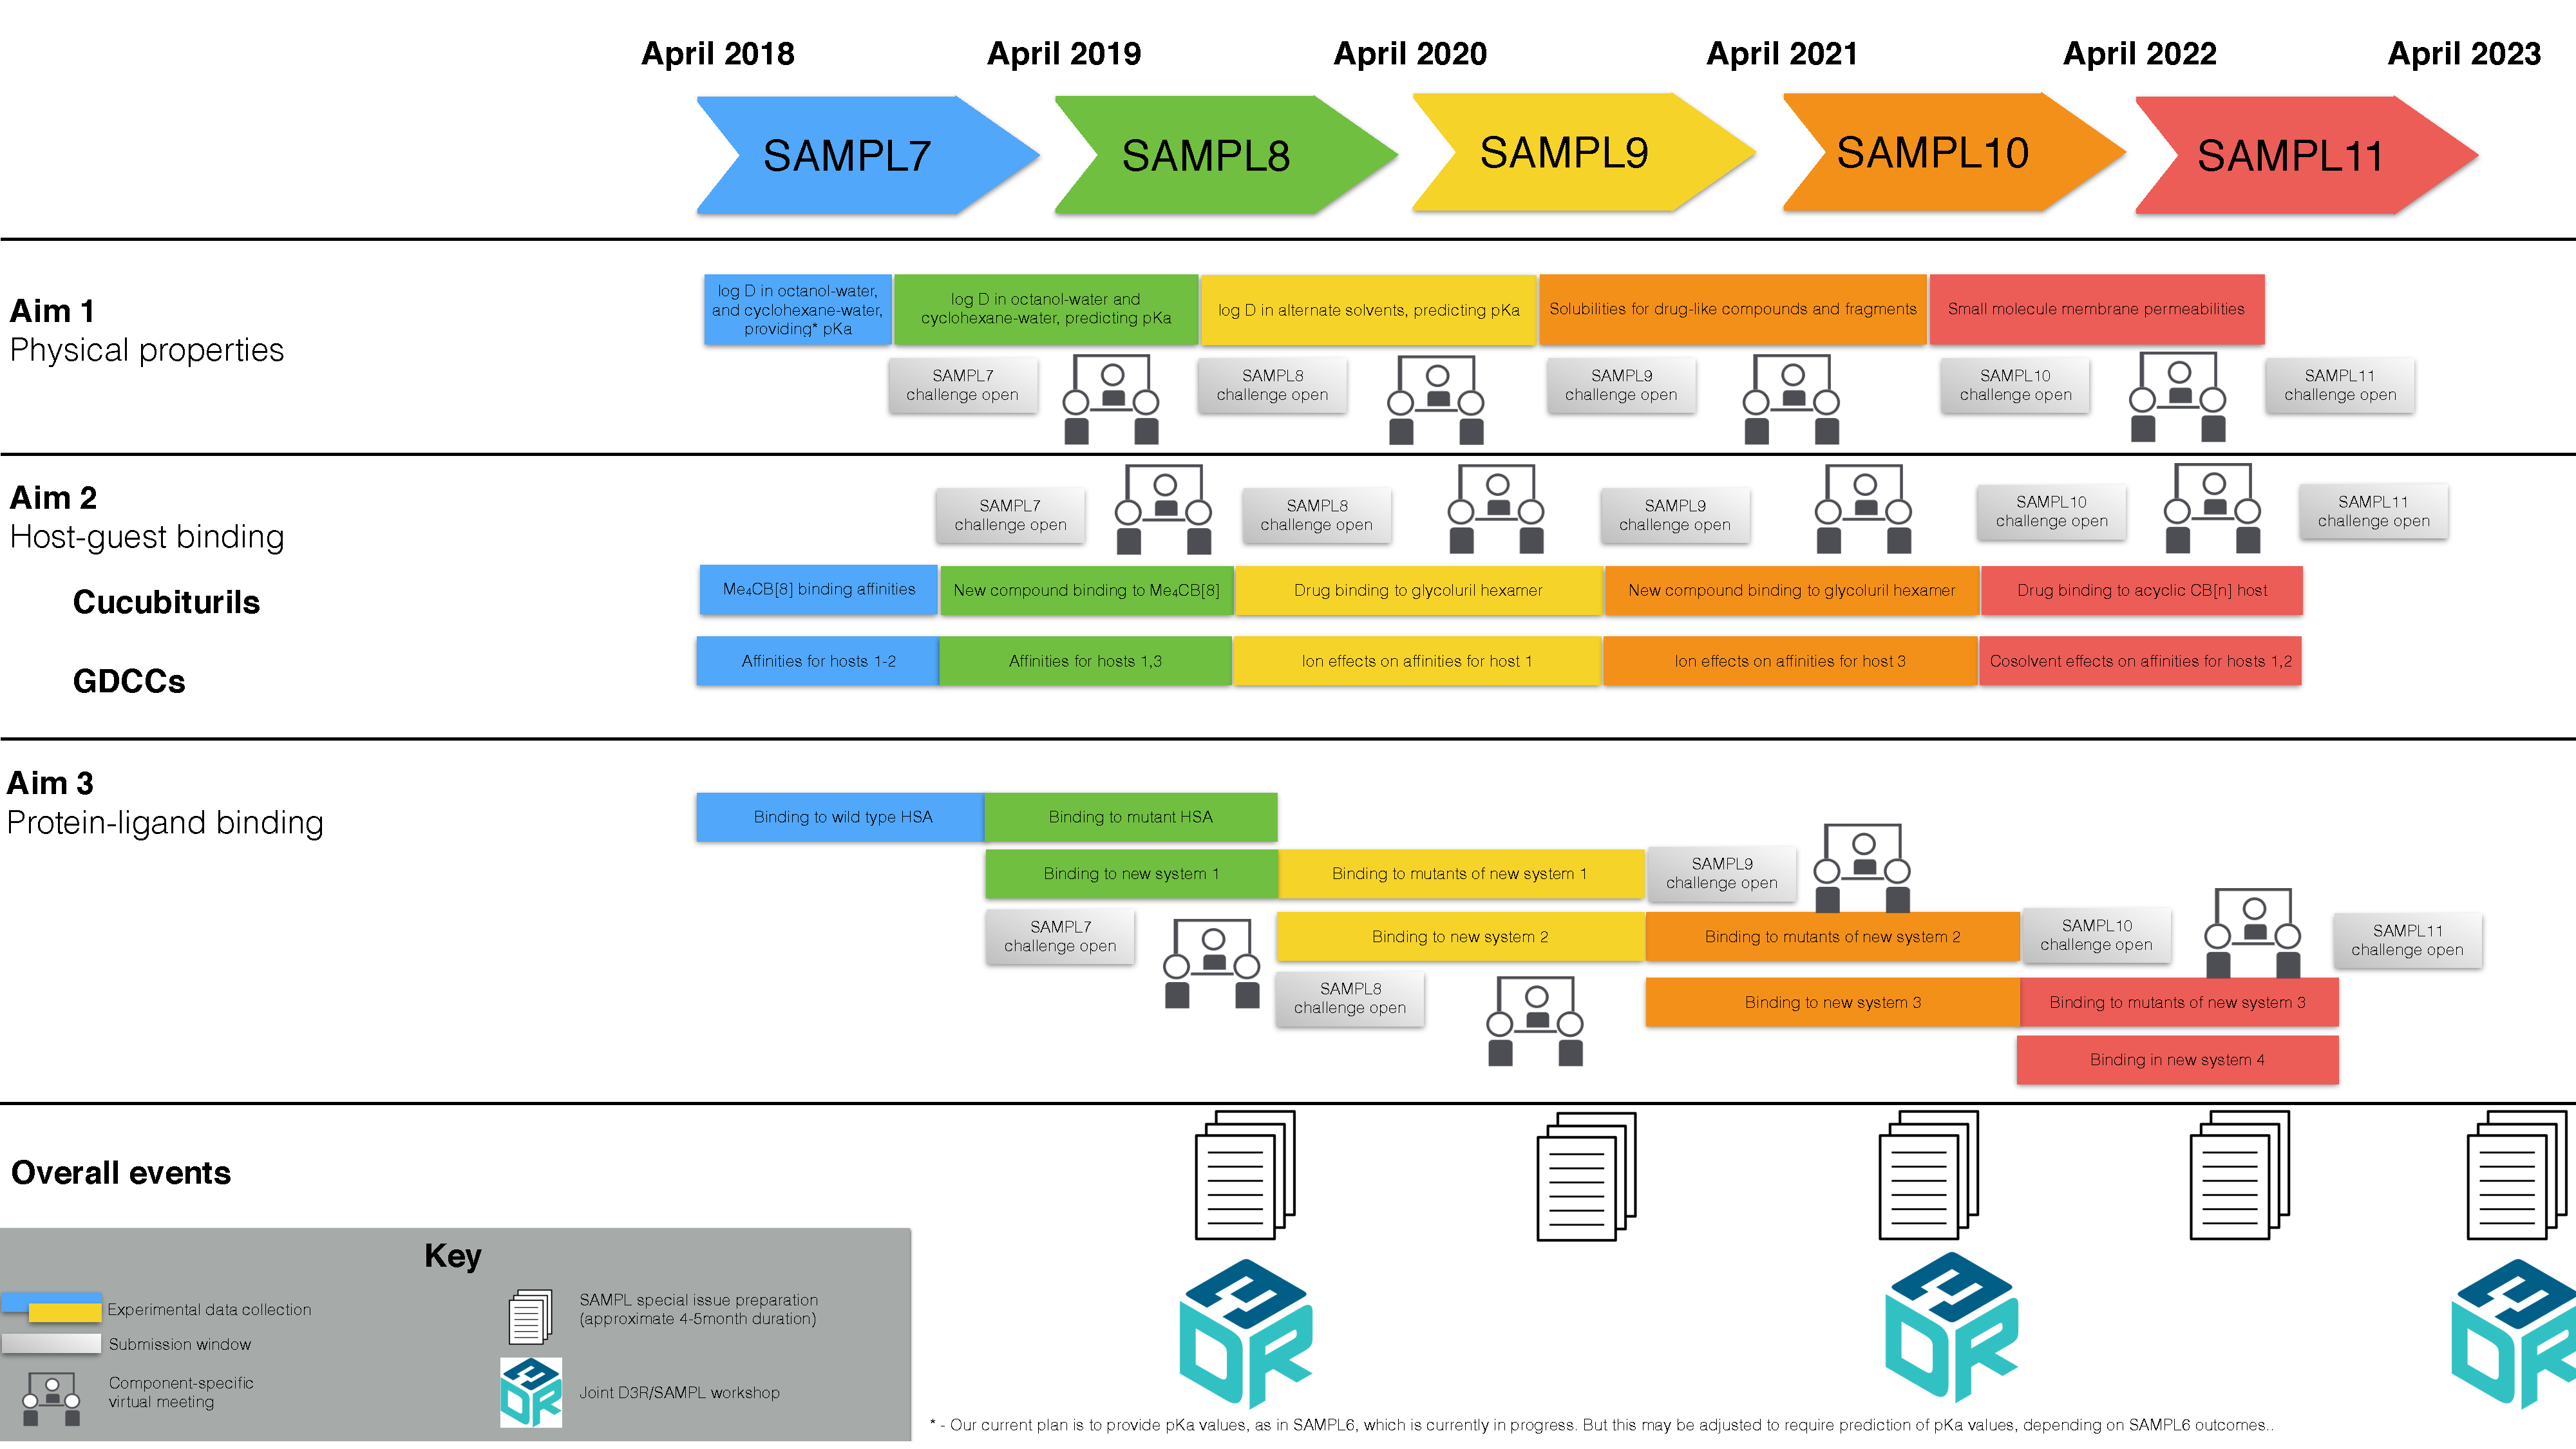
\includegraphics[width=\textwidth]{figures/Timeline3_cropped.pdf}
\end{centering}
\vspace{-0.25in}
\caption{\footnotesize {\bf Timeline for SAMPL activities.} Activities covered by this grant include data collection and SAMPL Challenges on our three major components (physical properties, host-guest binding, and protein-ligand binding), with each Challenge cycle color-coded separately.  
Data collection within each Aim is shown by a colored bar indicating what is measured and curated.
Data collection/curation is followed by a submission window for that Challenge component, then all results and analysis are returned to participants and posted on the SAMPL website; this also will nucleate more detailed long-term discussion on the relevant Slack channel.
At this point, we will also release the data to the public as a high quality benchmark.
Each component will then wrap up with a virtual meeting focused on lessons learned and areas which need further exploration; these will be recorded and posted on our website to assist in rapid dissemination of new insights. 
Virtual meetings precede the submission window for the next SAMPL Challenge, giving the opportunity to incorporate lessons learned for the next Challenge.
Submission windows and virtual meetings are staggered across categories so that participants can be involved in all three major areas without multiple simultaneous deadlines.
In-person meetings are co-hosted with D3R and will occur every two years, supplemented by effort-wide virtual meetings in between.
Special issues of JCAMD, where participants report lessons learned, will have deadlines shortly after the virtual meeting on the protein-ligand Challenge for that year, and a 4-5 month timeline (based on historical experience) from the submission deadline until the special issue appears (with the first papers appearing online substantially sooner).
Rapid dissemination is critical for rapid progress, so we encourage the use of preprints and informal reports to supplement the special issue.
\vspace{-0.25in}
\label{figure:timeline}}
\end{figure}
%%%%%%%%%%%%%%%%%%%%%%%%%%%%%%%%%%%%%%%%%%%%%%%%%%%%%%%%%%%%%%%%%%%%%%%%%%%%%%%%

{\Large \bf INNOVATION}

This work proposes a five-year plan for fielding SAMPL Challenges as an \emph{innovation engine} for molecular design.
Specifically, collaborative scientific competitions or Challenges are a proven model for inducing innovation~\cite{Saez-Rodriguez:2016:NatRevGenet, Kay:2011:R&DManage, Eisenstein:2013:NatBiotech}, applying crowdsourcing to finding and identifying robust new methodologies~\cite{Saez-Rodriguez:2016:NatRevGenet}. 
The proposed series of SAMPL Challenges brings crowdsourcing to bear on molecular interactions in a way which focuses on solving specific, incremental problems that impair our ability to accurately and robustly predict these interactions.
Thus, while the proposed work is indeed innovative (as we argue below), the most important innovation comes from participants in SAMPL Challenges, as is the case in all crowdsourcing approaches to innovation~\cite{Saez-Rodriguez:2016:NatRevGenet, Kay:2011:R&DManage}.

Reliance on others for innovation is a strength of this model. 
It is not always obvious where the most important innovations may come from, but Challenges draw together teams of diverse entrants, including unconventional innovators who may apply unorthodox, risky, or radical technologies~\cite{Kay:2011:R&DManage, Saez-Rodriguez:2016:NatRevGenet}; progress comes both from the usual suspects and unexpected sources.
It is not necessary to decide in advance who is best positioned to solve key problems~\cite{Saez-Rodriguez:2016:NatRevGenet}---the Challenge itself drives innovation and allows it to be recognized, regardless of source.

Crowdsourcing models for innovation have an ample track record, with the XPrize driving major headlines~\cite{::XPRIZE, Kay:2011:R&DManage, XPrize:2017:Wikipedia}, and the Netflix Prize also familiar to many~\cite{Bell:2010:CHANCE}. 
While there are other Challenges in the area of biomolecular modeling, such as D3R~\cite{Gathiaka:2016:JComputAidedMolDes}, the p$K_a$ cooperative~\cite{Nielsen:2011:Proteins}, CAPRI~\cite{Janin:2005:ProteinScience} and CASP~\cite{Moult:2014:Proteins},
\textbf{no other blind Challenge focuses specifically on datasets collected specifically to drive quantitative protein-ligand modeling}.

SAMPL is designed in the spirit of the wildly successful biomedical DREAM Challenge~\cite{Prill:2011:Sci.Signal., Eisenstein:2013:NatBiotech, Saez-Rodriguez:2016:NatRevGenet} which had more than 800 recent participants. 
As recommended by the DREAM Challenge organizers~\cite{Saez-Rodriguez:2016:NatRevGenet}, SAMPL focuses on high-quality data, decomposing complex problems into tractable but difficult component problems in order to benefit from crowdsourcing, and drawing together diverse teams and methods to allow various solutions to be evaluated.

\textbf{Our recent survey indicates SAMPL has already been important in advancing protein-ligand modeling}~\cite{Mobley:2017:eScholarship}; attached testimonials highlight some specific ways SAMPL has advanced science.
Several historical examples further serve to highlight how SAMPL can foster innovation (see also Figure~\ref{figure:sampl5_logD} and our SAMPL bibliography). 
While the first SAMPL Challenges focusing on hydration free energies saw heterogeneous performance, they highlighted pitfalls of existing methods and force fields which led to marked improvements in PB models~\cite{nicholls_samp1_2009, ellingson_analysis_2010,ellingson_efficient_2014}, identified some limitations of fixed-charge force fields~\cite{mobley_alchemical_2012, Fennell:2014:J.Phys.Chem.B} that spurred their repair~\cite{mobley_alchemical_2012, Fennell:2014:J.Phys.Chem.B, paranahewage_predicting_2016},
and helped motivate alternate implicit or hybrid solvent models~\cite{sulea_predicting_2011, li_testing_2014, brini_adapting_2016}.
Shifts in protonation state and tautomer proved particularly important in SAMPL5's log~D Challenge~\cite{Bannan:2016:JComputAidedMolDes, klamt_prediction_2016}, as they will in binding.
Host-guest binding Challenges~\cite{Mobley:2017:AnnualReviewofBiophysics}
have highlighted the importance of salt effects~\cite{yin_overview_2016, muddana_blind_2014, Mobley:2017:AnnualReviewofBiophysics}
and in some cases revealed severe force field limitations~\cite{yin_sampl5_2016, muddana_sampl4_2014-1}, pointing the way forward for improving predictive models~\cite{yin_toward_2015, Mobley:2017:AnnualReviewofBiophysics}.


%%%%%%%%%%%%%%%%%%%%%%%%%%%%%%%%%%%%%%%%%%%%%%%%%%%%%%%%%%%%%%%%%%%%%%%%%%%%%%%%
%SAMPL DC FIGURE
\begin{wrapfigure}[20]{r}[0pt]{9cm}
\vspace{-0.25in}
\begin{centering}
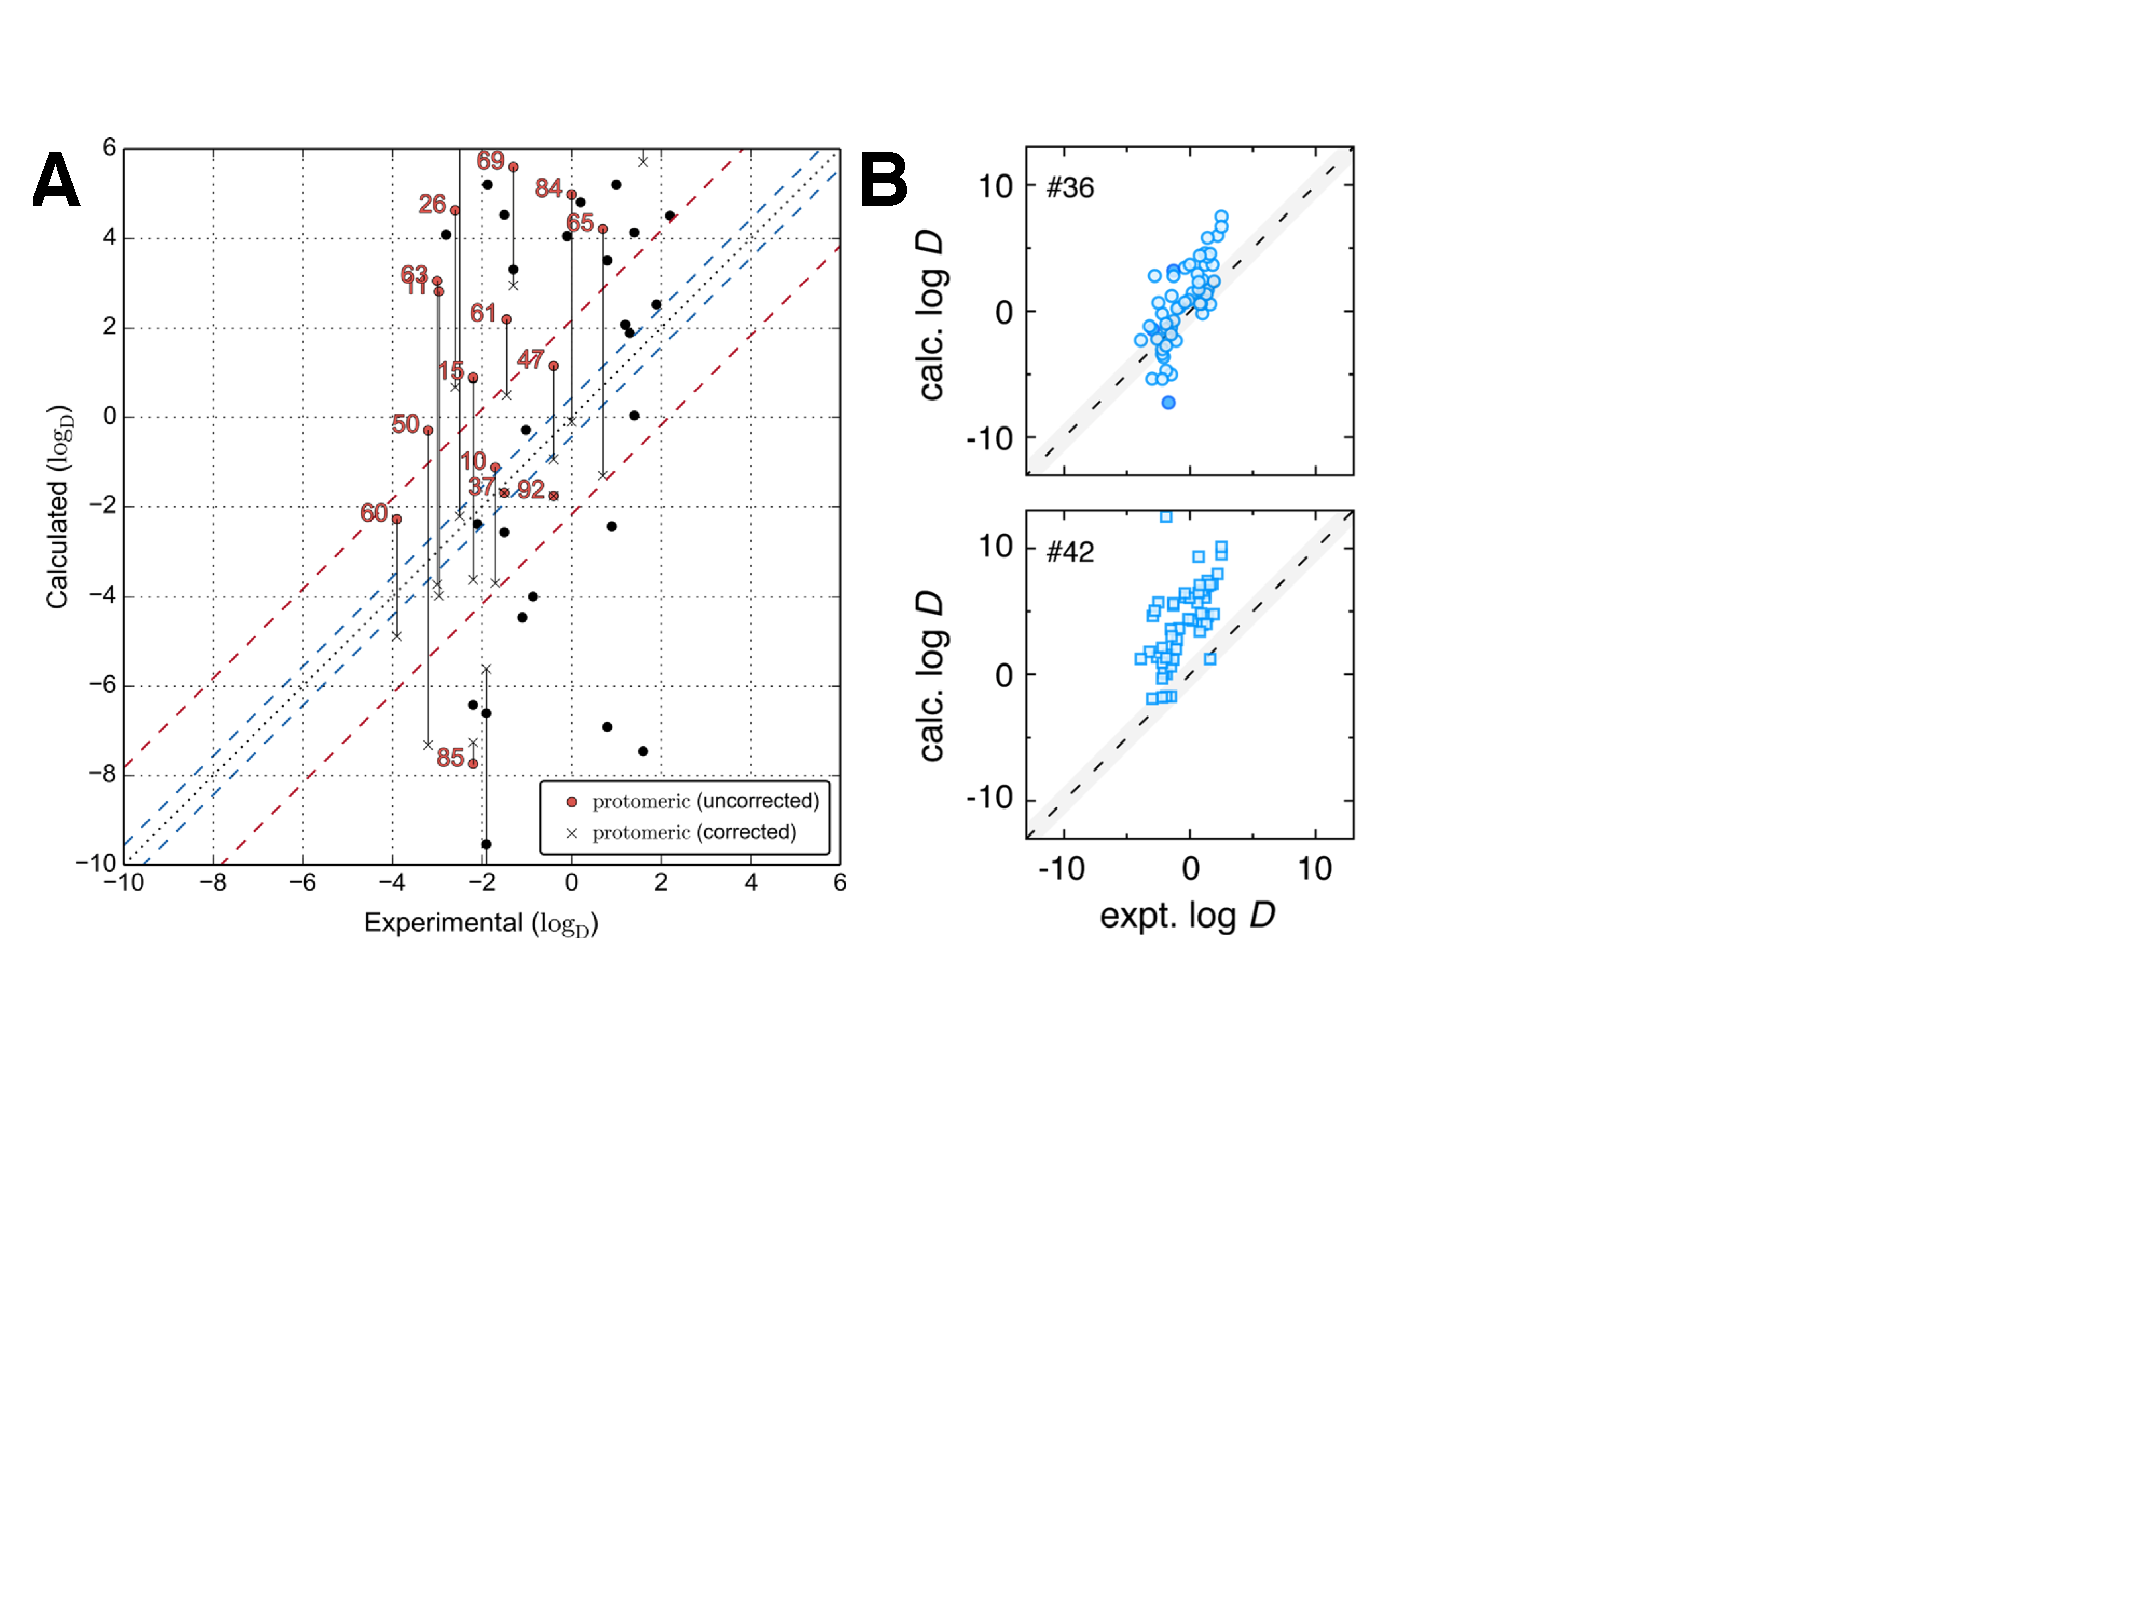
\includegraphics[width=\textwidth]{figures/sampl5_logD_v1.pdf}

\end{centering}
\footnotesize
\caption{\label{figure:sampl5_logD}  
\textbf{Lessons learned from SAMPL5 log~D predictions.} 
Predictions of log~D values for SAMPL5 provided a number of key lessons. (A) Methods which treated multiple protonation and tautomeric states in their predictions performed dramatically better than those which did not; here, red dots move to x symbols when these effects are treated, improving accuracy in every case~\cite{Pickard:2016:JComputAidedMolDes}. (B) Re-parameterization of a force field to more accurately reproduce pure solvent dielectric constants resulted in dramatically better predictions (top) than the original force field (bottom)~\cite{paranahewage_predicting_2016}. 
}
\end{wrapfigure}
%%%%%%%%%%%%%%%%%%%%%%%%%%%%%%%%%%%%%%%%%%%%%%%%%%%%%%%%%%%%%%%%%%%%%%%%%%%%%%%%

This proposal focuses on the development of SAMPL Challenges tailored to progressively advance computational methods for binding (Aim 4), gathering the requisite experimental data to drive these Challenges (Aims 1-3). 
\textbf{While the primary innovation will result from our Challenges, we also innovate on several other fronts.}
Aim 3 develops a new informatics platform to facilitate the rapid identification and study of useful protein-ligand systems that are both experimentally tractable for high-throughput biophysical measurement and focus on specific challenges of interest; an innovative, automated wetlab helps produce our high quality data. 
Additionally, students in our computational groups perform reference calculations to benchmark current state-of-the-art techniques.
This provides student training, but also drives innovation by (1) Benchmarking advanced community method entries against our reference ``current best practices'' calculations; (2) Facilitating learning by allowing others to compare against our reference results to determine how methodology differences impact results; and (3) Focusing the field on key issues by analyzing sensitivity to conditions such as ionic strength, protonation states or tautomers.

{\Large\textbf{APPROACH}}



\textbf{A series of data-driven Challenges will spur systematic advances in modeling for biomolecular design.}
We collect targeted experimental datasets focused on specific problems spanning a range of complexity (Aims 1--3), and use these to field SAMPL Challenges driving innovation (Aim 4).
%, with each Challenge including components from each of Aims 1--3.
Data collection brings together multiple laboratories and industrial collaborators, including both theorists and experimentalists: graduate students from the Mobley and Chodera laboratories are paired with well-equipped experimental groups in industry to collect physical property data (Aim 1); Gibb and Isaacs, leading experimentalists in supramolecular chemistry, work with theorist Mobley to perform host-guest affinity measurements (Aim 2); and the Chodera lab applies new automated approaches to identify suitable protein-ligand systems and measure binding (Aim 3).


\textbf{\underline{Aim 1: Collect new physical property datasets to assess accuracy and spur improvements in force fields}}\\
\textbf{\underline{and modeling of protonation states and tautomers.}} 


Simple physical properties such as solvation, phase partitioning, and protonation equilibria can be calculated precisely (but not necessarily accurately) with physical methods, allowing quantitative comparison between calculations and experiment and revealing and isolating deficiencies in our models. 
These properties allow us to directly probe force field accuracy and chemical effects like protonation and tautomer handling in the absence of slow conformational changes and other effects which complicate assessment in protein-ligand systems. 


{\bf Rationale:}
We will perform new solution-phase physical property measurements for drug-like molecules to motivate improvements in force fields and handling of protonation states and tautomers.
This builds on our work on water-cyclohexane distribution coefficients (log~D) for SAMPL5 (with Genentech), which revealed major issues with handling of protonation states and tautomers~\cite{Bannan:2016:JComputAidedMolDes} as well as serious force field limitations~\cite{paranahewage_predicting_2016} (Figure~\ref{figure:sampl5_logD}).
Distribution coefficients give the equilibrium ratio of solute concentration between aqueous and nonpolar phases at a given pH.
Thus, because these mimic transfer free energies from aqueous to protein- or membrane-like environments, they capture many of the same characteristics as binding but without the associated challenges of receptor conformational sampling and specific ligand-receptor interactions.
Many methods performed poorly in predicting log~D in SAMPL5, with even the best methods having accuracies less than would be expected based on hydration free energies~\cite{Bannan:2016:JComputAidedMolDes}, yet failures were informative and the major sources of error were issues which also plague ligand-receptor binding.
In many respects, distribution coefficients are an ideal SAMPL Challenge, as they are sufficiently difficult for clear failures to be frequent, with ample room for improvement, but not so difficult that reasons for failure were generally unclear. 
Still, many methods consistently disagreed with experiment for some compounds~\cite{paranahewage_predicting_2016, klamt_prediction_2016, Bannan:2016:JComputAidedMolDes, rustenburg_measuring_2016}, revealing the impact that targeted follow-up experiments (such as those we will conduct here) can have on improving models.
Thus, \textbf{targeted Challenges on solution-phase properties address some of the complexities of binding}.  

Previous physical property SAMPL Challenges have already driven significant progress, but a frequent request is for modestly larger datasets and follow-up experiments to re-check specific measurements~\cite{Mobley:2017:eScholarship}. 
This was impossible with donated data, but here, we will expand the size and quality of Challenge datasets, allowing us to expand to provide greater coverage of the full dynamic range. 
\textbf{Follow-up experiments will become routine, improving our ability to learn from failures.}
For example, SAMPL5's lack of dynamic range meant that, when calculated values often spanned a larger dynamic range than experiment, it was unclear if this was due to the choice of compounds, experimental limitations, or force field deficiencies~\cite{rustenburg_measuring_2016, Bannan:2016:JComputAidedMolDes, paranahewage_predicting_2016, klamt_prediction_2016}.  

{\bf Physical property datasets will be tailored for synergy with binding datasets.}
Specifically, ligands studied in host-guest and protein-ligand binding Challenges will be prioritized for inclusion in solution-phase physical property datasets; if physical property data is already public for these, analogs or fragments will be included. 
Thus, if a binding free energy proves difficult to predict, participants can determine if its solution-phase properties (such as protonation states or tautomers) were similarly difficult, thereby narrowing down the source of the error.

Below, we summarize plans for data collection for the SAMPL7-11 Challenges of Aim 4 (see also Figure~\ref{figure:timeline}).
These specific datasets were selected to help the field first resolve problems encountered in SAMPL5 and then progress to accurate estimation of additional properties.
Datasets will be larger than prior SAMPL Challenges---at least 96 compounds for good statistics---though when possible, a much larger amount of data will be collected.

\textbf{SAMPL7: Cyclohexane/water and octanol/water distribution coefficients, given pKa.}
Building on the success of distribution coefficients at motivating rapid modeling advances~\cite{Bannan:2016:JComputAidedMolDes}, we will measure cyclohexane-water distribution coefficients at pH 7.4 for a new batch of commercially-available drug- and fragment-like molecules overlapping with compounds studied in Aims 2 and 3.
We will also measure octanol-water distribution coefficients for the same compounds, given indications that their prediction may be computationally tractable~\cite{Bhatnagar:2013:PhysicalChemistryChemicalPhysics, bannan_calculating_2016} despite the heterogeneous structure of the wet octanol phase~\cite{Kollman:1996:AccountsofChemicalResearch}.
Because p$K_a$ prediction was difficult but critical for SAMPL5, we will focus SAMPL7 on force fields and tautomers by measuring and providing p$K_a$ values, revisiting p$K_a$ prediction in SAMPL8 and 9.
A similar approach is currently being applied for SAMPL6 (data collection is in process in collaboration with Merck), so plans here may be adjusted modestly depending on SAMPL6 outcomes.

\textbf{SAMPL8 and SAMPL9: Distribution coefficients and pKa's for drug-like molecules.} 
Distribution coefficient measurements conflate the challenging issues of protonation state and tautomer prediction, as well as transfer into different environments. 
After allowing participants to predict distribution coefficients given p$K_a$ values for SAMPL6-7, the SAMPL8-9 datasets will include distribution coefficients and p$K_a$ values, with participants asked to predict both. 
The datasets will include p$K_a$ values and distribution coefficients for an extensive set of drug-like molecules.
SAMPL8 will focus on octanol-water and cyclohexane-water, and SAMPL9 will shift to alternate solvents to ensure that models are capable of handling varied non-water phases. 
As in SAMPL7, we plan to focus partly on molecules and fragments overlapping with compounds being studied in Aims 2--3.

\textbf{SAMPL10-11: Solubility prediction and membrane permeability.}
With solubility predictions now becoming tractable~\cite{Schnieders:2012:J.Chem.TheoryComput., park_absolute_2014, liu_using_2016} (with Schr\"{o}dinger also working on amorphous solubility), solubility measurements will be a valuable test for SAMPL10, combining the solvation aspects of SAMPL1-8 with a new solid phase component.
New computational techniques are targeting membrane permeability~\cite{lee_permeability_2016, comer_permeability_2014}, and this is experimentally accessible (see support letters from Pfizer and Merck), leading to our interest in permeability for SAMPL11.
However, it is likely that both solubility and permeability will still be extremely challenging -- so we plan to also measure distribution coefficients and pKa's for the same compounds to help participants isolate potential points of failure.

Based on community feedback~\cite{Mobley:2017:eScholarship}, we are also interested in subsequent SAMPL Challenges on hydration and conformational free energies, and will seek suitable sources of reliable experimental data.

{\bf Experimental plan:}
Experimental data will be collected in collaboration with our pharma partners, roughly following the model used for SAMPL5, where Chodera lab student Bas Rustenburg worked with Genentech and adapted an existing workflow to measure cyclohexane-water log~D~\cite{rustenburg_measuring_2016}.
A similar approach is currently being employed with Merck for SAMPL6.
Thus, Mobley and Chodera lab students will visit industry partners collecting targeted datasets.
This collaborative approach (see Letters of Collaboration from Genentech, Pfizer, GSK, and Merck) gives us substantial access to equipment and high-throughput measurement workflows---such as the Sirius T3 (which can measure partition/distribution coefficients, p$K_a$s, and solubilities for molecules with titratable groups)---automation equipment, and compound libraries---for the purposes of rapidly collecting targeted datasets.
This approach works~\cite{rustenburg_measuring_2016}, and our partners see the value of this data and SAMPL to the community.

Overall, Aim 1 extends prior SAMPL Challenges via data focused on quantitative prediction of physical properties relevant to accurately predicting biomolecular interactions, paving the way to applications in more complex systems.

\eject

\textbf{\underline{Aim 2: Measure affinities of drug-like compounds in supramolecular hosts to challenge quantitative}}\\
\textbf{\underline{models of binding in systems not plagued by major receptor sampling issues.}}

%%%%%%%%%%%%%%%%%%%%%%%%%%%%%%%%%%%%%%%%%%%%%%%%%%%%%%%%%%%%%%%%%%%%%%%%%%%%%%%%
%SAMPL HG FIGURE
\begin{wrapfigure}[22]{l}[0pt]{7cm}
\vspace{-0.23in}
\begin{centering}
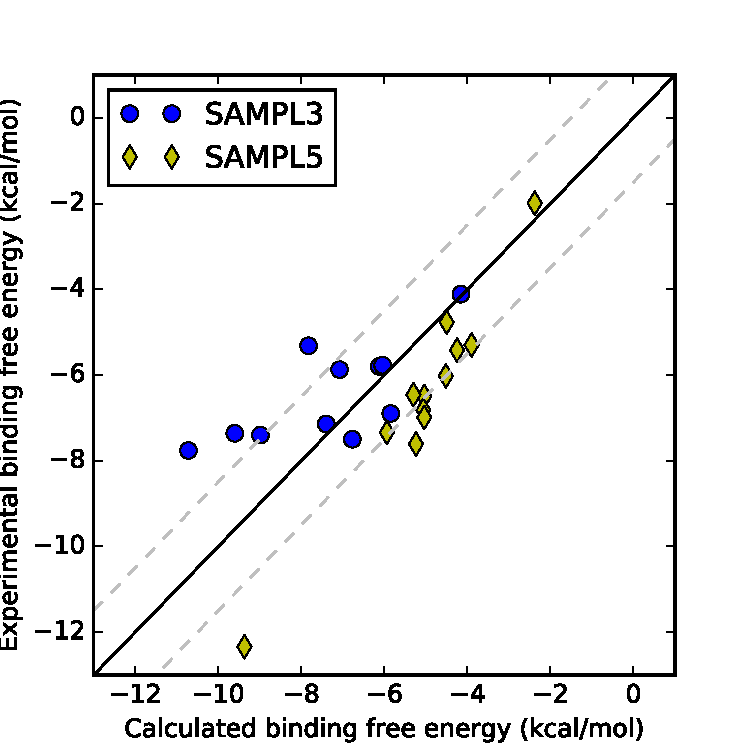
\includegraphics[width=\textwidth]{figures/sampl3_and_sampl5.pdf}

\vspace{-0.10in}
\end{centering}
\footnotesize
\caption{\label{figure:hg_sampl}  
\textbf{The best host-guest binding predictions of SAMPL3~\cite{muddana_sampl3_2012} and SAMPL5~\cite{yin_sampl5_2016}.} 
Binding free energy predictions have shown clear improvements from SAMPL3 to SAMPL5 as the major obstacles become understood and are treated better by models, though a systematic offset remains in the best SAMPL5 predictions (yellow). Dashed lines denote errors of $\pm1.5$ kcal/mol.
}
\end{wrapfigure}
%%%%%%%%%%%%%%%%%%%%%%%%%%%%%%%%%%%%%%%%%%%%%%%%%%%%%%%%%%%%%%%%%%%%%%%%%%%%%%%%

Moving beyond solution-phase physical properties, we want Challenge data which introduces some of the additional complexity of binding in a controlled manner.  
Aim 1 focuses on the behavior of small molecules in different environments, in the absence of receptors and the associated potential for slow sampling, strong specific interactions, and other challenges like salt effects.
Binding in host-guest systems (Aim 2) retains many of these same challenges and introduces strong specific interactions and other issues like salt effects~\cite{Mobley:2017:AnnualReviewofBiophysics}, while still avoiding many of the issues with slow sampling (of protein conformational changes, ions, and ligand binding modes) seen in biomolecular interactions.
\textbf{Thus, binding in host-guest systems introduces new challenges relevant to biomolecular interactions, but without the full complexity of protein-ligand interactions}, as recently reviewed~\cite{Mobley:2017:AnnualReviewofBiophysics}.

Already, host-guest SAMPL Challenges have provided key tests for modeling of binding interactions~\cite{Mobley:2017:AnnualReviewofBiophysics}, resulting in new attention paid to how co-solvents and ions modulate binding (resulting in errors of up to 5 kcal/mol when these effects are neglected) and the importance of adequately sampling water rearrangements~\cite{muddana_sampl4_2014, Mobley:2017:AnnualReviewofBiophysics, yin_overview_2016, bhakat_resolving_2016}.
This new attention has resulted in clear improvements (Figure~\ref{figure:hg_sampl}), though host-guest binding remains difficult to model accurately~\cite{henriksen_computational_2015}, in part due to force field limitations (resulting in new force field work~\cite{yin_toward_2015}).

\begin{wraptable}[18]{r}{6.5cm}
\vspace{-0.2in}
\footnotesize
\begin{tabular}{l | l}
{\bf drug} & {\bf features} \\
\hline
memantine & adamantane; 1:1 \\
saxagliptin & adamantane; 1:1 \\
premarin & steroid \\
pancuronium & steroid\\
varenicline & 1:1 vs 1:2 \\
valsartan & p$K_a$ 4.37 \\ 
omeprazole & p$K_a$ 4.77 \\
ranolazine & p$K_a$ 7.17; epitopes \\
pradaxa & p$K_a$ 3.87; epitopes \\
nilotinib & epitopes; p$K_a$ 6.3 \\
sensipar & epitopes; folding \\
vyvance & diamine; epitopes; folding \\
minocycline & tetracyclin; amino aniline \\
\end{tabular}
\caption{\textbf{\label{table:CB} Selected drugs whose binding to CB[$n$] hosts will be assayed for SAMPL7, 9, and 11 Challenges (SA 2.1).}  
These drugs bind to the cucubituril-based host systems considered here, some at high affinity, so measuring their affinities provides a way to test methods for predicting binding interactions absent complexities present in protein-ligand systems.
}
\vspace{-0.1in}
\end{wraptable}

Here, we design a series of SAMPL Challenges focused on two classes of host-guest systems---cucurbiturils and analogs (SA 2.1) and Gibb's deep-cavity cavitands (GDCCs, SA 2.2)---both of which build on prior SAMPLs.
These two sets of systems exhibit different complexities~\cite{Mobley:2017:AnnualReviewofBiophysics}, with the hosts of 2.1 bringing modest co-solvent and ion effects and some receptor sampling problems for the acyclic hosts, and the GDCCs of 2.2 bringing profound ion and co-solvent effects as well as water sampling challenges.
Methods which perform well on one class may not perform well on the other~\cite{Mobley:2017:AnnualReviewofBiophysics} because of these distinct challenges.
This diversity and complexity is important for Challenges which seek to drive researchers to focus on all of the important features rather than just a subset~\cite{Saez-Rodriguez:2016:NatRevGenet}.
As the SAMPL community would like even more diversity in hosts and guests~\cite{Mobley:2017:eScholarship}, we will also seek to include additional host-guest systems via data donation (as in SAMPL1-5).

SAMPL6 is currently in progress and includes components on GDCCs and cucubiturils, so our plans in this section may be adjusted somewhat depending on the outcomes of SAMPL6.

\textbf{Subaim 2.1: Cucurbituril-based receptors: model binding systems}

\textbf{Cucurbituril derivatives for host-guest binding.} 
Building on previous success with cucurbit[$n$]uril (CB[$n$]) experiments for SAMPL~\cite{ma_acyclic_2012-2, cao_absolute_2014, she_glycoluril-derived_2016}, we will conduct a series of new experiments on these receptors,
with experimental work conducted by co-investigator Isaacs, an expert on these systems who provided data for previous SAMPLs.
CB[$n$] receptors are particularly well suited to our goals because they exhibit: (1) strong binding affinities in water, comparable to protein-ligand affinities (routinely $\mu$M to nM; occasionally pM to fM)~\cite{cao_attomolar_2014, liu_cucurbituril_2005, mock_structure_1986, assaf_cucurbiturils:_2015, moghaddam_new_2011, shetty_can_2015, biedermann_release_2012}, (2) high selectivities between structurally related guests which translate into large $\Delta \Delta G$ values~\cite{isaacs_stimuli_2014}, (3) low molecular weights (1--2 kDa) permitting high levels of theory to be used, and (4) highly restricted conformational degrees of freedom, reducing conformational sampling challenges often seen in protein-ligand binding.
For SAMPL7-11, we will resynthesize a series of CB[$n$]-type receptors of increasing complexity, measure $K_a$ values, and determine host-guest stoichiometry and geometry toward pharmaceutically relevant guests (selected drugs) in order to stringently test methods for predicting binding.  
Figure~\ref{figure:CB} shows the chemical structures of three hosts---Me$_4$CB[8]~\cite{vinciguerra_synthesis_2015}, glycoluril hexamer~\cite{lucas_templated_2011}, and acyclic CB[$n$]-type receptors~\cite{ma_acyclic_2012, ma_acyclic_2012-1, zhang_acyclic_2014, gilberg_acyclic_2015, sigwalt_acyclic_2016, zhang_acyclic_2014-1} which span a range in terms of level of preorganization and formal charge.

\eject 

\textbf{SAMPL7-11 cucurbituril Challenges.} 


\begin{figure}[h]
\vspace{-0.1in}
\begin{centering}
\resizebox{\textwidth}{!}{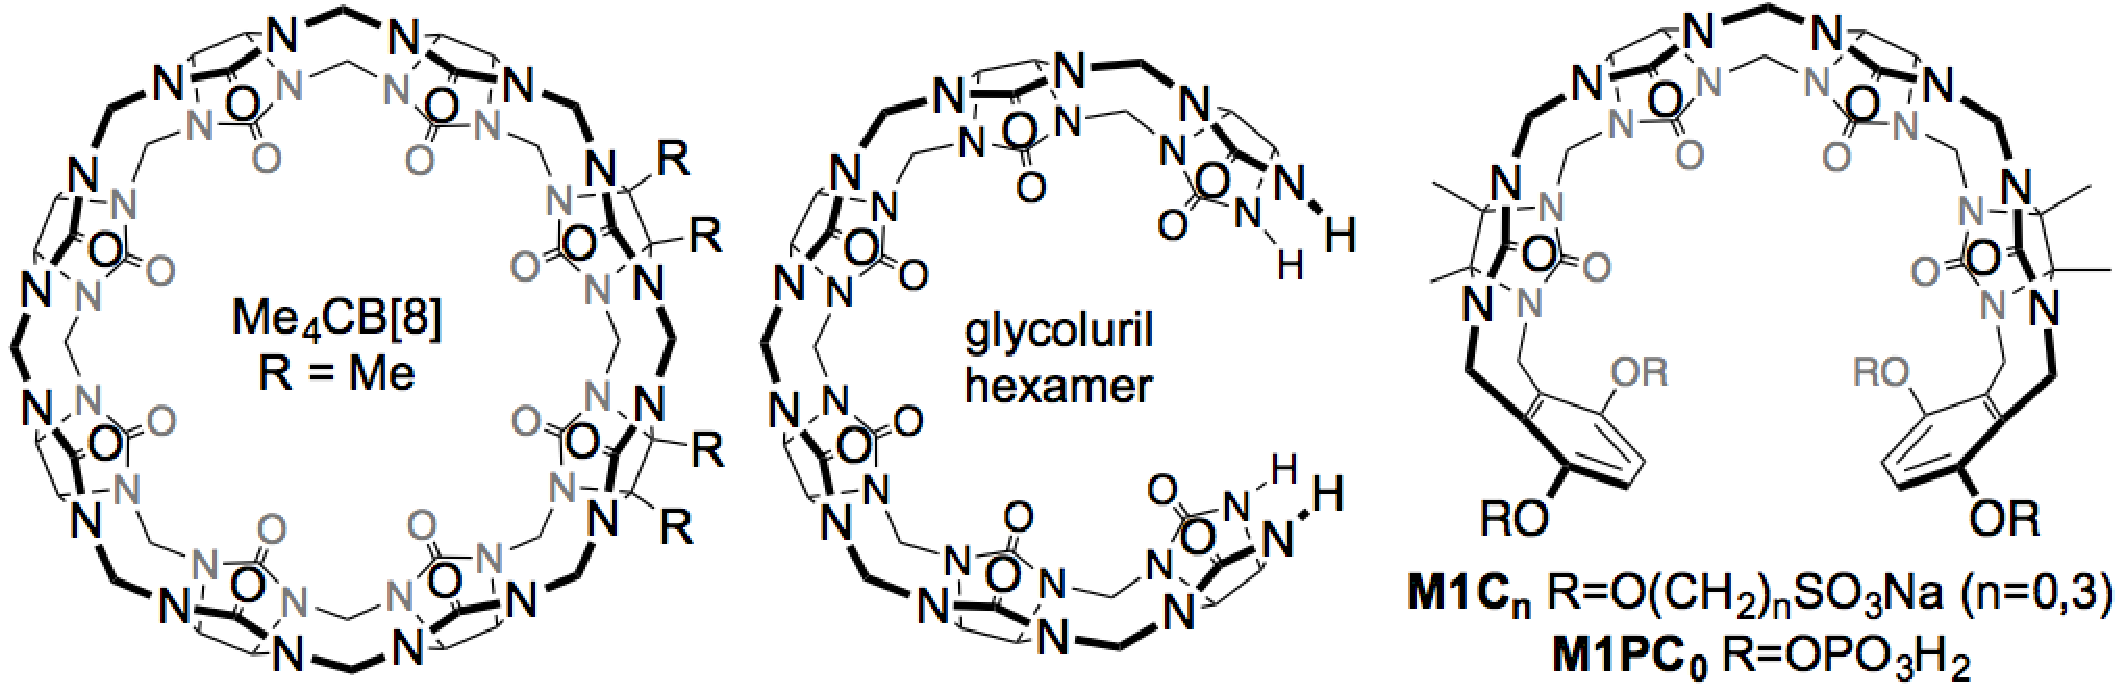
\includegraphics{figures/CB.pdf}}

\end{centering}

\caption{
\label{figure:CB} \footnotesize {\bf SAMPL7-11 host-guest Challenges will feature cucubituril hosts and analogs, including Me$_4$CB[8], glycoluril hexamer, and acyclic CB[n]-type receptors (SA 2.1).} 
These receptors bind a variety of drug-like molecules, some with high affinity.
\vspace{-0.15in}
}
\end{figure}


\emph{For SAMPL7}, we will measure $K_a$ and $\Delta H$ values, stoichiometry, and geometry for the interaction of Me$_4$CB[8] (a soluble CB[8] derivative) with 15 guests (selected top drugs, Table~\ref{table:CB}) by either direct or competition isothermal titration calorimetry (ITC), UV/Vis or fluorescence indicator displacement assay, or NMR competition experiments, as previously~\cite{cao_attomolar_2014, liu_cucurbituril_2005, ma_acyclic_2010, she_glycoluril-derived_2016}.  
Our selection of Me$_4$CB[8] binding to top drugs allows us to modulate the computational complexity by: 1) changing host flexibility (e.g. Me$_4$CB[8] can exhibit ellipsoidal deformation)~\cite{vinciguerra_synthesis_2015}, 2) allowing the possibility of binary or ternary (e.g. 1:1 and/or 1:2 host:guest) complexes~\cite{ko_supramolecular_2007, barrow_cucurbituril-based_2015, urbach_molecular_2011}, 3) using drugs with several potential binding epitopes or modes to induce sampling issues.  
Host:guest stoichiometry and geometry (e.g., which binding epitope is complexed) will be addressed by ITC $n$ values, Job plots monitored by UV/Vis or NMR~\cite{connors_binding_1987}, and by $^1$H NMR complexation induced changes in chemical shifts~\cite{masson_cucurbituril_2012}.  
All studies will be conducted in phosphate buffered saline (p$H$ 7.4 with physiological salt) which introduces its own complexities due to salt competition for binding~\cite{marquez_mechanism_2004, Mobley:2017:AnnualReviewofBiophysics}. 
\emph{SAMPL8} will revisit the same host, but use 15 different guests be selected from commercial sources on the basis of reference calculations (on a larger set of guests) to ensure that they cover substantial dynamic range and/or exhibit affinities that depend substantially on the force field or water model, thus effectively testing our force fields and methods.
For \emph{SAMPL9}, we will focus on binding of the same 15 drugs (Table~\ref{table:CB}), but to glycoluril hexamer. 
This host introduces the complication of increased conformational dynamics, and influences the number and energy of solvating (and unusually coordinated) water molecules implicated in the high binding constants for CB[$n$]-guest complexes~\cite{biedermann_release_2012, biedermann_hydrophobic_2014}.  
The selected drugs include several with p$K_a$ values in the 3.8 to 7.4 range; given that CB[$n$]-type receptors (like biomolecular receptors) can induce p$K_a$ shifts in their guests of up to 4 p$K_a$ units~\cite{saleh_activation_2008, nau_deep_2011, ghosh_strategic_2012}, this will test how well models can predict these effects. 
Additionally, it will couple nicely with the focus on p$K_a$ values in Aim 1 -- especially so given that Aim 1 compound will include some of the same chemical functionality.
\emph{SAMPL10} will revisit glycouril hexamer with the same 15 guests from \emph{SAMPL7}.
\emph{SAMPL11} will shift to acyclic CB[$n$]-type receptors (e.g. M1C$_3$, M1C$_0$, and M1PC$_0$ that contain anionic solubilizing groups attached via different linker lengths.  
As in SAMPL3~\cite{muddana_sampl3_2012}, these acyclic CB[$n$]-type receptors introduce conformational complexity, and water interactions play a key role.

\textbf{Subaim 2.2. Gibb deep cavity cavitands for host-guest studies} 

{\bf History of GDCC SAMPL Challenges.} During SAMPL4~\cite{gibb_binding_2013} and SAMPL5~\cite{sullivan_binding_2016} we focused on two specific GDCC hosts: the octa-acid 1 (R = H) and another octa-acid variant with four methyl groups at the portal of the binding pocket (1, R = Me). 
These studies used ITC to measure the thermodynamics of (1) host {\bf 1} (R = H) binding a range of 9 carboxylate guests,
and (2) the binding of 6 carboxylate and trimethylammonium guests to both hosts ({\bf 1}, R = H and Me; Figure~\ref{figure:gdccs}).  
In both cases $^1$H-NMR titration was also used to confirm ITC-derived free energies of binding.  
Relative to cucubiturils, the GDCCs introduce new complexities because of their tight exit portal, modest issues with host conformational sampling, slow water rearrangements, salt/buffer condition-dependence, and protonation state complexities~\cite{Mobley:2017:AnnualReviewofBiophysics, yin_overview_2016}.
Thus GDCC-oriented Challenges are particularly important since these issues complicate protein-ligand interactions as well.

{\bf Novel deep cavity hosts probe the effects of binding site charge constellations.} 
For future GDCC datasets, we will expand on the range of hosts by including {\bf 2} and {\bf 3} in our ITC studies (Figure~\ref{figure:gdccs}).  
Like cavitand {\bf 1}, host {\bf 2} is an octa-acid derivative.  
However, the four benzoate groups are relocated from the extreme exterior in the case of {\bf 1}, to the rim of the binding pocket in {\bf 2}.  
This is expected to have a direct effect on the binding of charged guests as well as an indirect effect on guest complexation via changes to the solvation of the empty host.  
Octa-trimethylammonuim cavitand (``positand'' {\bf 3}) has the same overall architecture as host {\bf 1}, but inverts the charges on the water solubilizing exterior coat.  
While it is not yet clear if this switch in groups relatively remote from the pocket will directly affect guest complexation, results from related systems suggest it can (unpublished). 

\begin{figure}[h]
\vspace{-0.1in}
\begin{centering}
\resizebox{\textwidth}{!}{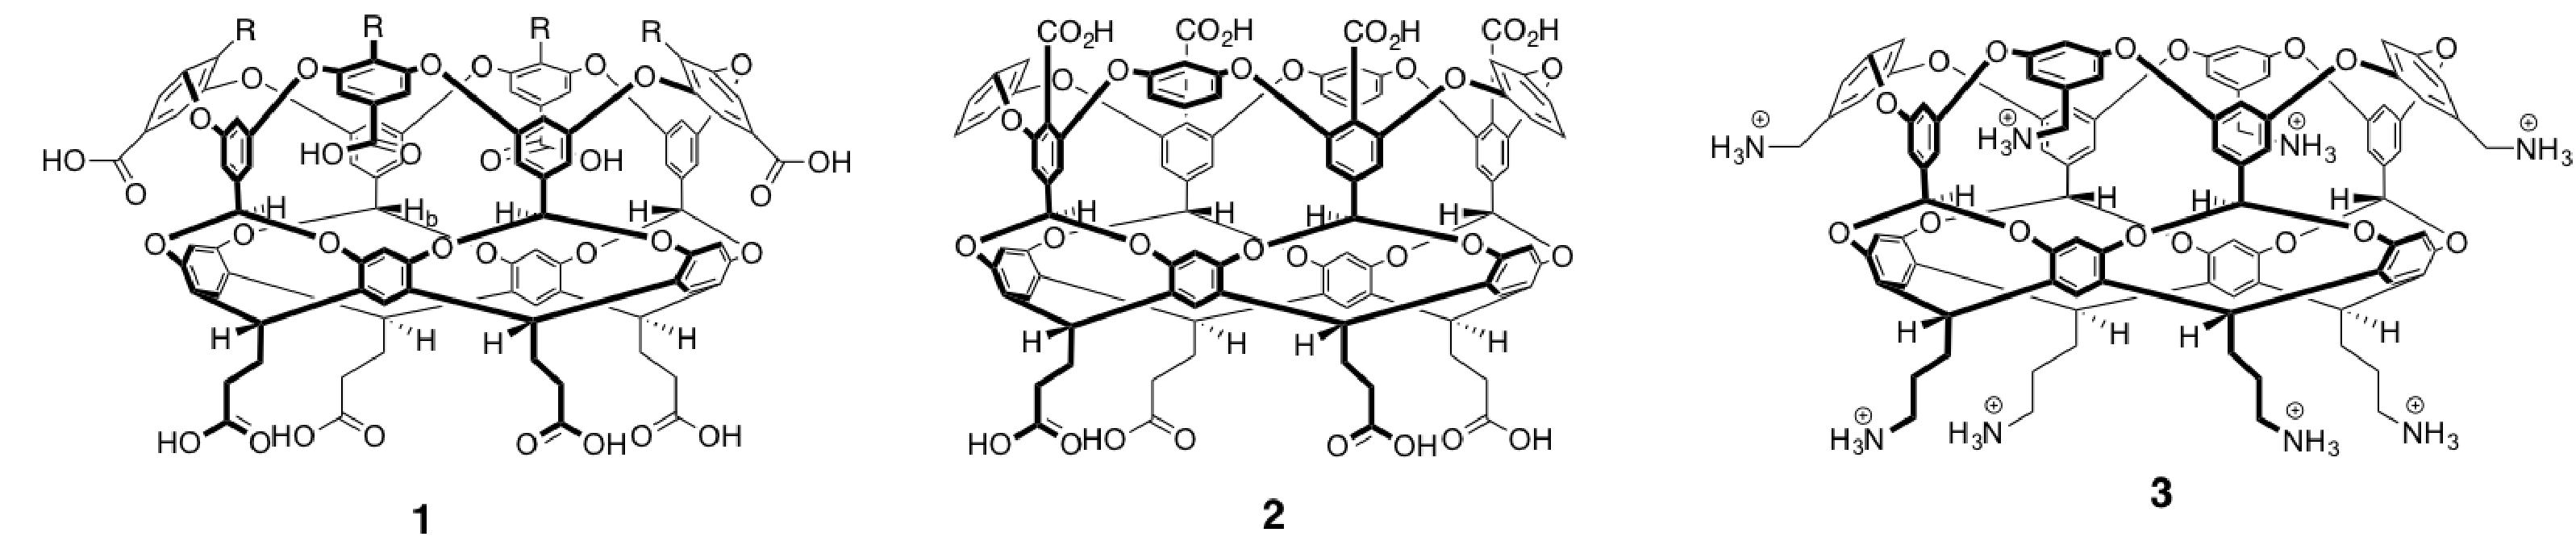
\includegraphics{figures/gdccs.pdf}}

\end{centering}

\vspace{-0.15in}
\caption{\footnotesize {\bf Gibb deep cavity cavitands for the SAMPL7-11 datasets (SA 2.2).} These hosts bind a variety of carboxylate and trimethylammonium guests in a strongly salt-dependent manner, providing a stringent test of our ability to model salt-dependent binding.
\label{figure:gdccs}
\vspace{-0.1in}
}
\end{figure}

{\bf SAMPL7-11 deep cavity cavitand datasets.} 
Data for SAMPL7 will focus on how well the effect of host carboxylate substituent location can be predicted, and will involve hosts {\bf 1} and {\bf 2} with a set of at least five previously uninvestigated guests.  
Guests will be selected from commercial sources on the basis of reference calculations in a similar manner to SAMPL8 in Subaim 2.1, specifically picking guests which have broad dynamic range and, here, have marked differences in affinities between hosts.
SAMPL8 will provide a second iteration of this experiment to test algorithmic improvements in predictive modeling following SAMPL7 by comparing hosts {\bf 1} and {\bf 3} with a different set of guests.  
We anticipate that because of the relative remoteness of the charged groups in these two hosts, the effects of switching charges will be subtler than the differences between {\bf 1} and {\bf 2}.  
SAMPL9 will consider the effect of common biologically-relevant counterions/salts on guest binding, comparing the effects of NaCl and NaI on the complexation of at least five guests to {\bf 1}.  
We have previously shown that iodide has a weak affinity for the binding pocket of {\bf 1}, while sodium ions have an affinity for the outer carboxylates~\cite{carnegie_anion_2014}, requiring modeling to capture the differential affinities of these ions in addition to guest affinities to successfully model the observed affinities.  
SAMPL10 will follow up on this by examining the effects of these same two salts on the complexation of at least five guests to {\bf 3}, again giving the modeling community time to incorporate algorithmic improvements following SAMPL9. 
While we have not yet quantified salt affinities to host {\bf 3}, we expect the iodide to have affinity for both the pocket and the positively charged solubilizing groups.  
For SAMPL11 we will consider the effects of co-solvents on the binding of five guests to {\bf 1} and {\bf 2} to probe the effect of co-solvent competition for the binding site, as well as effects co-solvents may have on weakening the hydrophobic effect. 
Participants frequently request larger datasets, so every effort will be made to include additional guests beyond the minimal number proposed if time allows or if human time can be reduced (such as via automated calorimetry).
Regardless, the total number of binding affinities measured for the family is substantial, so the data will be of considerable value as a benchmark~\cite{Mobley:2017:AnnualReviewofBiophysics}. 


\textbf{\underline{Aim 3: Develop model protein-ligand systems that isolate specific modeling challenges of drug targets.}}

To drive real improvement in quantitative modeling of protein-ligand interactions, we need to be able to revisit the same systems again and again in order to gauge and drive progress---in much the same way as participants in the Netflix Challenge had to genuinely improve their ability to predict user feedback to succeed~\cite{Bell:2010:CHANCE}.
While D3R~\cite{Gathiaka:2016:JComputAidedMolDes} evaluates the accuracy of current protein-ligand binding methods, performance in each Challenge iteration varies widely depending on the nature of the donated pharmaceutical data and difficulty of the target.
The high complexities of D3R targets make it difficult to identify clear points of failure~\cite{ignjatovic_binding-affinity_2016, deng_large_2016, sunseri_d3r_2016, Gathiaka:2016:JComputAidedMolDes}.
For example, while kinases are targets of great interest to drug discovery, blind Challenges involving kinase targets conflate issues of slow protein conformational dynamics~\cite{Lin:2013:Proc.Natl.Acad.Sci.}, protonation state effects of protein~\cite{Shan:2009:PNAS} and ligand~\cite{Szakacs:2005:JournalofMedicinalChemistry,Grante:2014:SpectrochimicaActaPartA:MolecularandBiomolecularSpectroscopy}, phosphorylation, charged ligands, and other challenges; failures on such targets are thus often unexplained. 

Only by revisiting the same systems repeatedly will we benefit from the wisdom of the crowds in identifying specific problems and validating solutions to these problems. 
Thus, here, {\bf we identify and develop model protein-ligand systems to \emph{isolate} specific accuracy-limiting effects in a series of SAMPL Challenges.}
By developing \emph{model binding systems}---biological protein-ligand systems comprised of single-domain proteins binding to a simple ligand series free of complex phenomena---we can study systems of complexity intermediate between completely artificial systems (like the valuable T4 lysozyme L99A model binding site~\cite{mobley_predicting_2007,merski_homologous_2015, Mobley:2017:AnnualReviewofBiophysics}) and complex pharmaceutical targets where multiple modeling challenges make it difficult to learn from failure (Figure~\ref{figure:mining-for-model-systems}A).
This allows Challenges focused on identifying and evaluating multiple solutions to selected accuracy-limiting effects (such as how to deal with ligand and protein protonation-state issues~\cite{Onufriev:2013:QuarterlyReviewsofBiophysics}, slow protein conformational dynamics, etc.), with the ability to revisit the same systems repeatedly as needed to drive innovation.

%%%%%%%%%%%%%%%%%%%%%%%%%%%%%%%%%%%%%%%%%%%%%%%%%%%%%%%%%%%%%%%%%%%%%%%%%%%%%%%%
% FIGURE: HSA SAMPL7 CHALLENGE
%%%%%%%%%%%%%%%%%%%%%%%%%%%%%%%%%%%%%%%%%%%%%%%%%%%%%%%%%%%%%%%%%%%%%%%%%%%%%%%%
\begin{figure}[h]
\begin{centering}
\resizebox{\textwidth}{!}{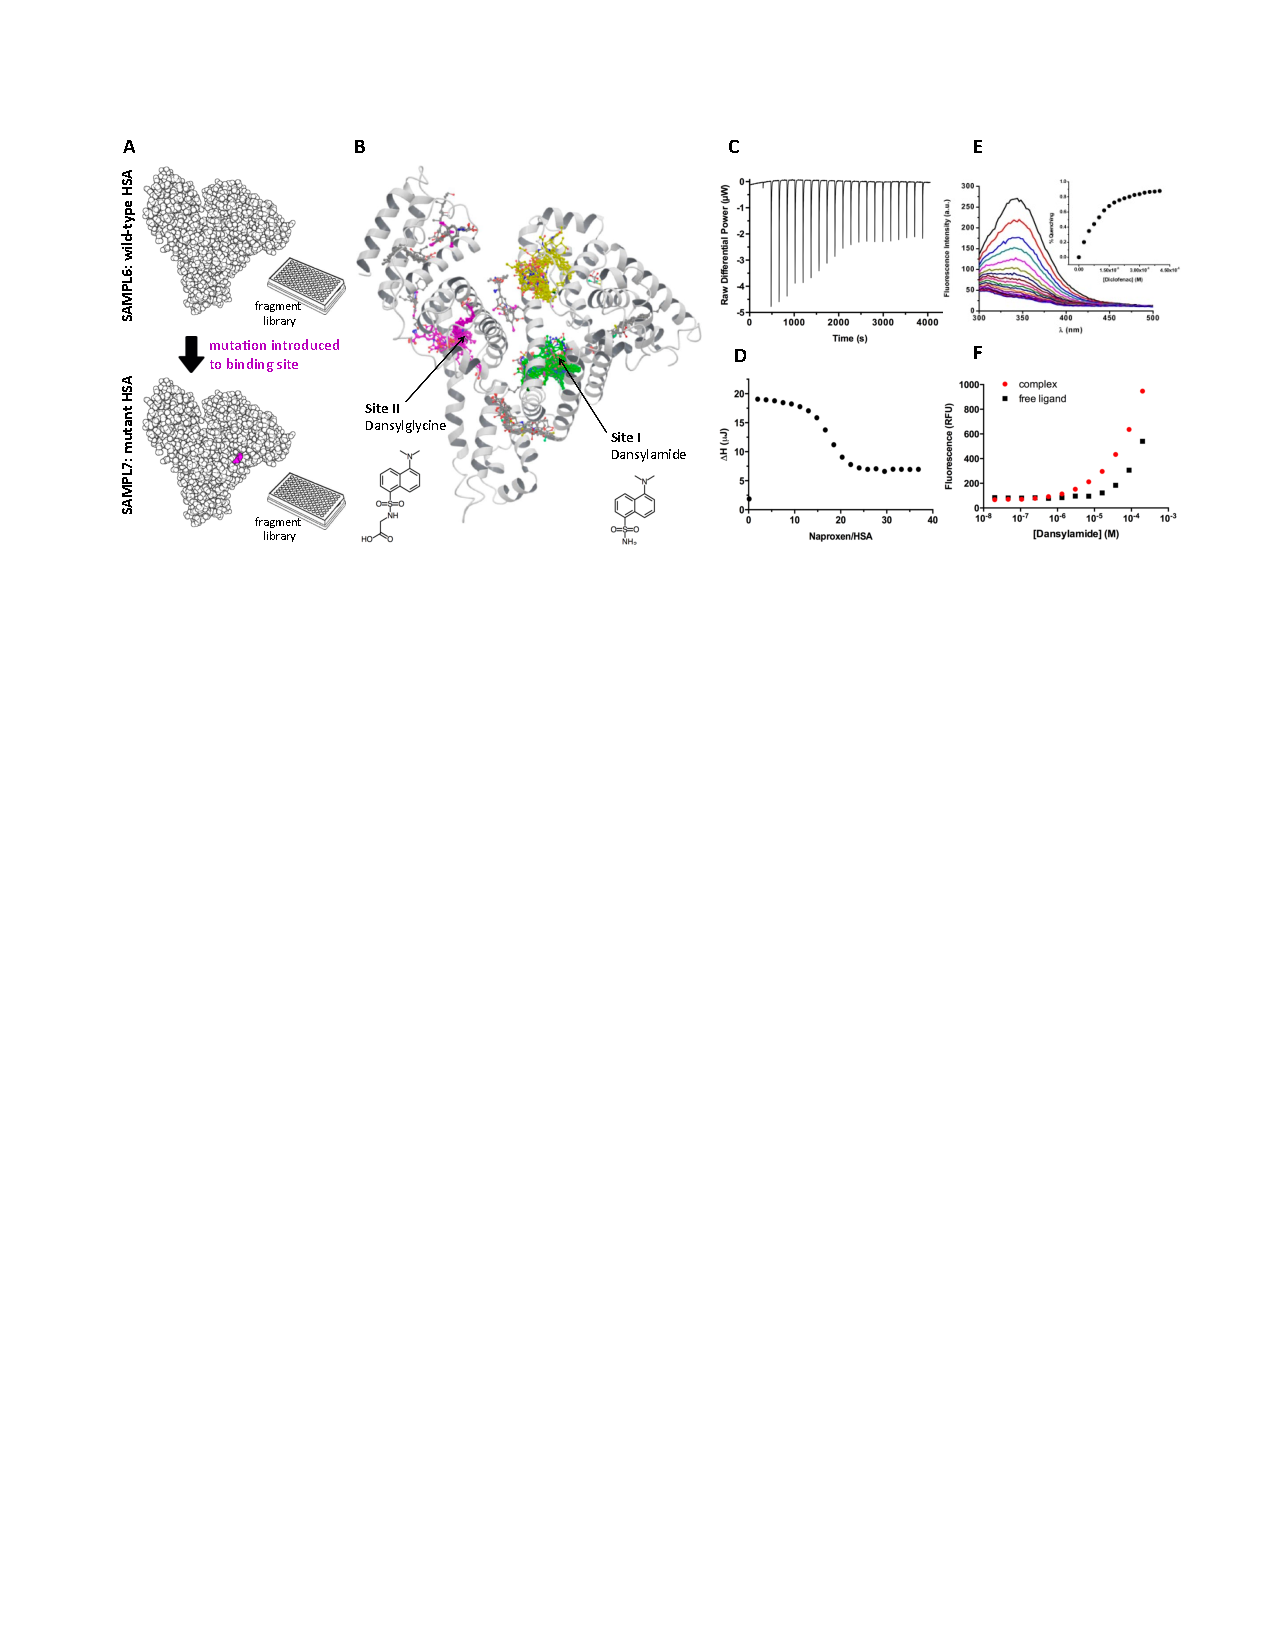
\includegraphics{figures/hsa-figure-draft7.pdf}}

\end{centering}
\vspace{-0.1in}
\caption{\footnotesize {\bf The SAMPL7/8 protein-ligand Challenge focuses on soluble drug fragment binding to human serum albumin (HSA) (Aim 3).}
\emph{(A)}~SAMPL7 will study binding of a library of at least 96 small soluble druglike fragments to recombinant HSA, with an engineered HSA mutant used for SAMPL8.
\emph{(B)}~HSA has at least eight known binding sites, with two major well-characterized sites (green, Sudlow's Site I; purple, Site II) that bind a variety of drugs (figure from~\cite{Hall:2013:JournalofChemicalInformationandModeling}).
Two fluorescent probes---dansylamide and dansylglycine---bind with $\sim$$\mu$M affinity and high selectivity to Site I and Site II, respectively; both exhibit binding-enhanced fluorescence at 480 nm, and can be used to site-specifically probe ligand affinities by competition.
\emph{(C, D)}~Binding affinities of soluble molecules can be measured by isothermal titration calorimetry (ITC); here, we show the \emph{(C)} differential power and \emph{(D)} integrated injection heats for the ITC titration of HSA by naproxen sodium collected using the Chodera lab automation pipeline;
\emph{(E)}~HSA tryptophan fluorescence quenching can also be used to measure ligand binding affinity; here, HSA titration by diclofenac is shown, with the inset plot showing percent quenching at 346 nm~\cite{Epps:1999:JournalofPharmacyandPharmacology,Bou-Abdallah:2016:TheJournalofChemicalThermodynamics}.
\emph{(F)}~Direct fluorescence binding assay of Dansylamide (fluorescent ligand) and HSA collected on the Chodera lab automation system. 
The binding curve can be constructed based on binding-induced fluorescence emission at 480 nm.
\vspace{-0.15in}
\label{figure:hsa-challenge}}
\end{figure}
%%%%%%%%%%%%%%%%%%%%%%%%%%%%%%%%%%%%%%%%%%%%%%%%%%%%%%%%%%%%%%%%%%%%%%%%%%%%%%%%

Crowdsourced innovation enhances the potential of model systems for driving progress.
For example, SAMPL3 focused on charged fragments binding to trypsin~\cite{Newman:2011:JComputAidedMolDes}, and rapidly focused the field on the deficiencies of current alchemical free energy methodologies in treating the binding of charged ligands.
Within two years, multiple laboratories developed solutions to this problem~\cite{Rocklin:2013:TheJournalofChemicalPhysics, lin_overview_2014, Reif:2014:JournalofComputationalChemistry}.

\textbf{SAMPL7-11 model protein-ligand Challenges.} 
We will introduce a new model protein-ligand system each SAMPL (revisiting the prior SAMPL's system if this becomes too difficult), with multiple Challenges on each system (Figure~\ref{figure:timeline}) to allow iterative improvement and assessment.
Our SAMPL7 data will focus on the binding of small soluble drug fragments to one particular protein (below), with fragments also studied in Aim 1. 
However, maximizing gains in this area requires adapting subsequent Challenges based on deficiencies identified by prior Challenges, so our new informatics platform (below) will aid in system selection.

\textbf{SAMPL7: Assessing predictive modeling of binding to multiple weak sites via measuring fragment binding to human serum albumin (HSA).}
HSA, the most abundant blood plasma protein, has a remarkable ability to bind a variety of small molecule drugs in multiple binding sites (Figure~\ref{figure:hsa-challenge}B)~\cite{Fasano:2005:IUBMBLife(InternationalUnionofBiochemistryandMolecularBiology:Life)}.
Using HSA as a model receptor isolates the challenge of multiple weak ligands binding to a stable rigid protein that is also pharmacologically relevant because of its dramatic modulation of drug pharmacokinetics~\cite{Hall:2013:JournalofChemicalInformationandModeling}.
HSA has at least \emph{eight} known binding sites, with numerous crystal structures available for drugs binding to two predominant sites (Site I and II)~\cite{Hall:2013:JournalofChemicalInformationandModeling}.
Small soluble molecules resembling drug fragments are highly likely to bind to HSA ($\ge$90\% of such fragments, as detected by SPR~\cite{Elinder:2011:JournalofBiomolecularScreening}), providing an experimentally-tractable diverse set of ligands spanning several orders of magnitude in affinity~\cite{Elinder:2011:JournalofBiomolecularScreening}.
As many current physical modeling methods assume a single well-defined binding site with high affinity~\cite{Gilson:1997:BiophysicalJournal}, this Challenge will allow the isolation of the effect of weak multiple binding from the majority of other confounding factors in protein-ligand binding.
HSA is relatively rigid, and computational methods already show some promise in computing binding affinities to HSA~\cite{Hall:2013:JournalofChemicalInformationandModeling,Lexa:2014:PLoSONE,Evoli:2016:Phys.Chem.Chem.Phys.}, making this an optimal model system.

Recombinant HSA will be expressed in \emph{E.~coli} and purified via refolding from inclusion bodies~\cite{Latta:1987:Bio/Technology}, then defatted at low pH~\cite{Lang:2015:BiotechnologyProgress} to ensure the resulting protein is free of the glycosylation and bound fatty acids found in plasma-isolated HSA~\cite{Lang:2015:BiotechnologyProgress}.
Recombinant expression will allow mutant forms of HSA (engineered via single-primer mutagenesis) to be fielded for SAMPL8 (Figure~\ref{figure:hsa-challenge}).
We will obtain a diverse library of at least 96 soluble drug-fragment-like molecules in pre-plated format as dry compound, and use our automated ITC pipeline (Figure~\ref{figure:hsa-challenge}C,D) to characterize overall binding affinities to HSA.
The same ligands pre-plated in DMSO format will be used to conduct a separate set of fluorescence titration assays (monitoring tryptophan fluorescence quenching, Figure~\ref{figure:hsa-challenge}D) and competition assays with site-specific fluorescent probes (Figure~\ref{figure:hsa-challenge}B) to resolve site-specific affinities to Sites I and II.
We will field several levels of Challenges, including Challenges focused on affinities to Sites I and II, as well as Challenges focused on predicting overall affinity and stoichiometry.

\textbf{SAMPL8-11: Rapid development of new tailored model systems using a novel informatics platform.} We are developing a novel informatics platform, TargetExplorer, to identify protein targets that can be rapidly developed into tractable model systems focusing on individual challenges (Figure~\ref{figure:mining-for-model-systems}).
This tool filters all known protein targets with structural data available in the PDB, first selecting for experimental tractability, then annotating experimentally tractable targets to determine which targets possess (or are likely to be free of) specific challenges for physical modeling.
This will allow us to select systems isolating specific modeling challenges.

%%%%%%%%%%%%%%%%%%%%%%%%%%%%%%%%%%%%%%%%%%%%%%%%%%%%%%%%%%%%%%%%%%%%%%%%%%%%%%%%
\begin{wrapfigure}[37]{r}[0pt]{9.5cm}
\vspace{-0.25in}
\begin{centering}
\resizebox{9.0cm}{!}{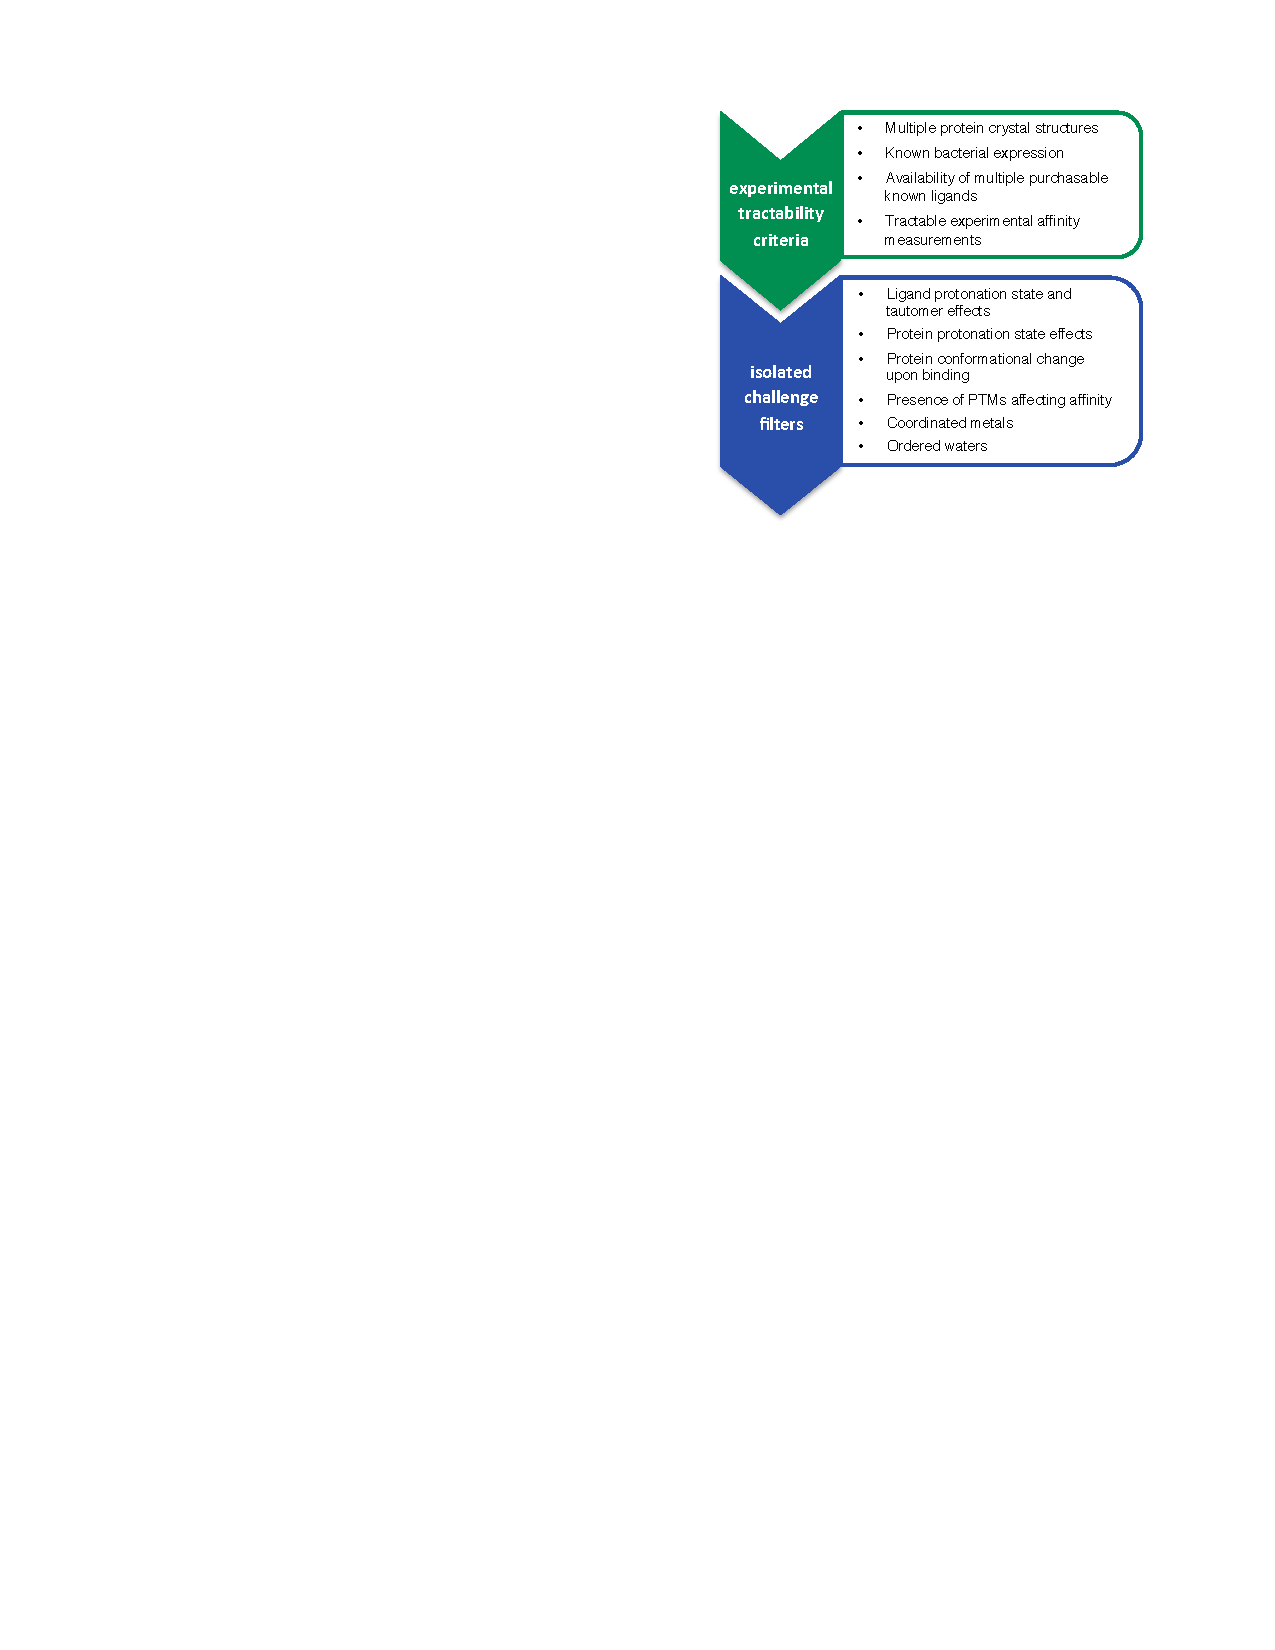
\includegraphics{figures/model-systems-figure-draft4.pdf}}
\vspace{-0.15in}
\end{centering}
\footnotesize
\caption{\label{figure:mining-for-model-systems}  
\textbf{Mining model protein-ligand systems to focus on individual modeling challenges via a structural and chemical informatics platform (Aim 3).}
We are developing a structural and chemical informatics system called TargetExplorer [\url{https://github.com/choderalab/targetexplorer}] that applies successive filters to all potential protein-ligand systems for which structural data is available. 
Suitable model systems should meet all experimental tractability criteria (green box) and possess only a few challenging properties, ideally only one (blue box).
Tractability of experimental affinity measurements includes properties like known ligands with potentially fluorescent scaffolds (for fluorescence competition assays), highly soluble ligands (for ITC), or ligands above a minimal mass (for SPR or MST).
Additional filters annotate experimentally tractable systems with their potential computational challenges, including charged ligands or potential ligand protonation state or tautomer effects~\cite{Martin:2009:JournalofComputer-AidedMolecularDesign} (deduced from predicted aqueous protonation/tautomer energies); potential protein protonation state effects (deduced from MCCE2 calculations~\cite{Song:2009:JournalofComputationalChemistry}); protein conformational changes (deduced from variation in protein conformation or the presence of unresolved loops in protein-ligand crystal structures); the presence of post-translational modifications that may affect affinity (deduced from Uniprot annotations); coordinated metals (identified in crystal structures); and ordered waters (present in multiple crystal structures).
}
\end{wrapfigure}
%%%%%%%%%%%%%%%%%%%%%%%%%%%%%%%%%%%%%%%%%%%%%%%%%%%%%%%%%%%%%%%%%%%%%%%%%%%%%%%%

The Chodera lab has developed an automated wetlab to facilitate the development of such systems using bacterial expression (see Equipment and Facilities).
Potential targets matching desired challenge criteria will be screened for bacterial expression using high-throughput cloning, transformation, and expression testing, with purity and yield assessed by capillary electrophoresis on a Caliper GXII.
Targets will be screened for stability in various buffers using Thermofluor thermal shift assays~\cite{Reinhard:2013:ActaCrystallographicaSectionFStructuralBiologyandCrystallizationCommunications}.
Ligands identified via TargetExplorer as spanning a wide dynamic range of binding affinities will be purchased as dry powder stocks and prepared for assay by highly accurate gravimetric solution preparation techniques using a Quantos automated balance.
Our lab has access to a wide variety of biophysical techniques for measuring protein-ligand binding affinities, including fluorescence (if fluorescent probe ligands are available), absorption (e.g.~Soret band shifts), automated isothermal titration calorimetry (provided ligands are sufficiently soluble), surface plasmon resonance, microscale thermophoresis (MST), luminescence, and alphascreen; all except MST are fully automated. 

We take a twofold approach to developing Challenge datasets:
First, we will purchase and assay small molecules similar to known ligands, presuming that these molecules are likely to have measurable affinities.
Second, using single-primer quick-change mutagenesis, we will introduce site-directed mutants to modulate the binding affinities of known ligands.
This can be performed and screened for expression in 96-well format.
Thus, datasets will consist of a matrix of protein mutants and ligands, providing opportunity to deeply explore the effects of interest.

\textbf{\underline{Aim 4: Crowdsource innovation via community}}\\
\textbf{\underline{blind Challenges to advance biomolecular design.}}\\
The heart of our work lies here -- driving innovation via community blind SAMPL Challenges centered around the datasets of Aims 1---3 (Figure~\ref{figure:timeline}).
This approach utilizes crowdsourcing (see Innovation, above) to advance science.
Our Challenges test the state of the art, provoke new methodological and force field innovations, allow comparative evaluation of methods so that advances are quickly recognized and spread, and drive downstream improvements.
Our SAMPL Challenges are progressive, building on one another so that for success in later Challenges, participants must build on lessons learned from prior Challenges.
Each iteration will likely yield its own incremental benefits (e.g.. as in Figure~\ref{figure:sampl5_logD}) for molecular design, in addition to contributing to progress towards accurate prediction of biomolecular interactions.

\textbf{SAMPL blind Challenges.} Yearly SAMPL Challenges following our timeline (Figure~\ref{figure:timeline}) serve to advance the state-of-the-art.
As is critical for such Challenges~\cite{Saez-Rodriguez:2016:NatRevGenet}, we will advertise aggressively via press releases, commentaries in relevant journals, CCL, e-mail, and Twitter. 
As experimental data for each component becomes available and is curated, input files and Challenge details will be made available at least six months prior to the Challenge deadline; data not yet available at that time will be held for a subsequent Challenge (with the exception of three months for year 1 due to startup timescales).
Advertising will feature our full timeline (which will also be available at \url{https://drugdesigndata.org/about/sampl} along with details of plans) allowing planning of participation. 
Challenge datasets will now also be larger than prior SAMPLs, as frequently requested~\cite{Mobley:2017:eScholarship}. 


As in prior SAMPLs, submissions will be handled by a web upload service on the SAMPL website which validates submissions to ensure that they meet format standards for automated processing and analysis. 
Analysis will be conducted by our automated Python framework, and results returned automatically online.
All participant submissions and methodology descriptions will (as before) be made available publicly on the website, along with participant information (except for participants who specifically request to remain anonymous prior to submission).
Aggregate statistics and historical performance will also be made available on our website, along with a record linking publications to historical submissions.

As the project progresses, we will push to transition towards submission of \emph{methods} rather than of \emph{predictions}. 
Specifically, as automated workflow engines such as OpenEye's Orion, AutoDesk's MDT, and others begin to be adopted on a larger scale, we will push participants to submit their methods in a standardized package, and automatically apply their submitted method to the Challenge data via cloud computing resources.
This is already done in some Challenge platforms~\cite{Saez-Rodriguez:2016:NatRevGenet} but will be new to SAMPL, resolving one major hurdle for participation. 
Participants, while enthusiastic about SAMPL and how it benefits science, often note the burden of participating~\cite{Mobley:2017:eScholarship}; submission of methods rather than results will solve this problem, allowing participation with minimal investment of human time.
This will also allow for easy archival of methods and a focus on testing workflows rather than human expertise.
We will work with the NSF-funded Molecular Sciences Software Sustainability Institute (MolSSI) to identify best practices in this respect. 
One hurdle will be obtaining computer time, but we will seek donations of time from cloud computing vendors, support from pharma, and adapt our workflows so we can run on NSF supercomputing resources where we will seek grants. 
In the worst case we would ask participants submitting methods for a modest budget to run their methods, but having this level of automation results in substantial savings in human time which can itself result in monetary savings. 
This migration will also facilitate post-Challenge follow-up and method comparison, by allowing us to archive reproducible methods.
Technology already allows this sort of archival and reproducibility, such as via Docker~\cite{docker_what_2015} containers with the participants' executable programs~\cite{Saez-Rodriguez:2016:NatRevGenet}.


\textbf{We will leverage SAMPL Challenges to identify modeling failures and identify potential solutions.} 
The learning process begins prior to each Challenge and continues afterwards. 
In advance,  we provide guidance to participants as to what known modeling issues we expect may be relevant.
For a host-guest system, for example, we might highlight known buffer/salt effects, protonation state challenges, and point out previous work on sampling challenges, with pointers to the relevant experimental work and to modeling work from past SAMPL Challenges and elsewhere~\cite{Mobley:2017:AnnualReviewofBiophysics}.
This helps participants design their approach.
{\bf Additionally, we will run reference calculations using current best practices.} 
This serves several purposes:
It provides a test of the current methods and force fields; it helps facilitate learning---we announce what calculations we plan to perform, make input files available in a wide variety of formats~\cite{shirts_lessons_2016, yin_overview_2016, Bannan:2016:JComputAidedMolDes}, and others can repeat our calculations with with method or force field variations to test protocol differences; it provides training to our students who are involved (as these reference calculations provide them familiarity with the latest methods and make them instrumental in community learning);  and it allows sensitivity analysis, as by varying the conditions (protonation state, tautomer, etc.,~\cite{Bannan:2016:JComputAidedMolDes}) we can see how much this impacts calculated values and thereby how important each factor is.
Reference calculations have, for example, helped us highlight the importance of a small amount of water in cyclohexane for accurately calculating log~D values, show how an incorrect tautomer could affect calculated values by many log units~\cite{Bannan:2016:JComputAidedMolDes}, and discover that small force field modifications could significantly improve results on hydration free energies~\cite{mobley_blind_2014-1}.

{\bf Dissemination of Challenge results.}
The most critical phase of each Challenge occurs after results are released. 
Typically, some participants uncover specific problems or solutions which are missed by others, so dissemination of these insights becomes critical to drive improvements.
SAMPL workshops will occur after Challenges every two years (years 1, 3, and 5), co-hosted with D3R Grand Challenge workshops (see support letter)
During the off years, discussion and dissemination of results will be via asynchronous means (below) and a ``virtual workshop'' consisting of talks and interaction over Google Hangouts or YouTube Live.
For all workshops, virtual or otherwise, talks will be selected from abstracts written to describe what each participant learned from participating---allowing us to prioritize presentations from those who have learned a great deal or done exceptionally well, rather than those who are simply testing an existing method with no new insight gained. 
If the D3R effort is not renewed, we will run SAMPL workshops independently, controlling costs via the model we use for our Workshops on Free Energy Methods in Drug Design---specifically, most participants will pay their own way to the workshop, and we will seek pharmaceutical and software industry sponsorships to defray costs. 

Rapid dissemination of results is critical so that new insights can be used in subsequent Challenges.
We will continue to publish special issues of the \emph{Journal of Computer Aided Molecular Design} (JCAMD) collecting publications related to each year's SAMPL Challenges (see Letter of Support).
As requested by participants~\cite{Mobley:2017:eScholarship}, we will also begin providing summaries of the key results and insights from each SAMPL that are suitable for a broad, non-technical audience -- either in JCAMD or as commentary in another suitable journal.
To ensure immediate availability of reports, we will strongly encourage prepublication sharing of results and analysis, including both slides and posters from SAMPL meetings (via F1000 Research) and paper preprints (via bioRxiv).

Post-Challenge analysis also drives progress, and often occurs outside of formal workshops and meetings.
While this has happened in the past---for example, when participants using similar methods work together after the SAMPL meeting to identify the origin of these discrepancies~\cite{monroe_converging_2014, yin_overview_2016, bhakat_resolving_2016, bosisio_blinded_2016, Mobley:2017:AnnualReviewofBiophysics}---we hope to accelerate this kind of collaboration.
To facilitate rapid exchange of ideas and open communication between the community, we will use collaboration software---such as Slack, which facilitates scientific communication for the NASA/JPL Mars Rover teams and NSF antarctic scientific research teams---to build a community discussion platform, 
facilitating a process of learning from one another more rapidly than normal publication channels. 
Given the overlap between molecules/fragments used in Aim 1 and those studied in Aims 2--3, insights from one Challenge component will have implications for predictions in the other components, making this rapid exchange key.
The students supported in this project will also play a role, working to understand the methods employed and bringing together researchers using similar methods to try and understand performance differences, including by running follow-up calculations.  


\textbf{Each Challenge will have lasting effects}.
SAMPL datasets are collected primarily to drive Challenges, but both the datasets and the lessons learned have lasting value.
The lessons learned will have the most immediate near-term impact and are critical for progress because each Challenge builds on prior iterations. 
However, the datasets themselves are also key.
In the past, due to the unfunded nature of SAMPL, we primarily emphasized compilation of the datasets and conducting Challenges. 
However, SAMPL datasets achieved a life of their own outside of SAMPL, becoming standard test sets~\cite{Mobley:2014:JComputAidedMolDes, DuarteRamosMatos:2017:J.Chem.Eng.Data, Mobley:2017:AnnualReviewofBiophysics, Yang:2017:arXiv:1705.10035[q-bio], Gosink:2017:J.Phys.Chem.B}.
This is one way SAMPL Challenges achieve their lasting effect, so we will perform additional curation on datasets post-Challenge, with follow-up experiments (as often requested by participants~\cite{Mobley:2017:eScholarship}) when needed, then release the data publicly as standard benchmark sets~\cite{Mobley:2017:AnnualReviewofBiophysics}.
We will make the data (including primary data, processed data, and our analysis of Challenge submissions) available freely and publicly with permanent, citeable DOIs; ensure relevant data is deposited in standard community repositories (e.g.~BindingDB~\cite{Liu:2007:Nucl.AcidsRes.}); and guarantee data longevity via backup hosting on library archival facilities (such as the UC's DASH (\url{https://dash.cdlib.org/})).



%%%%%%%%%%%%%%%%%%%%%%%%%%%%%%%%%%%%%%%%%%%%%%%%%%%%%%%%%%%%%%%%%%%%%%%%%%%%%%%%%%%%%%%%%%%%%%%%%%%%%%
% COLLABORATION MANAGEMENT PLAN
%%%%%%%%%%%%%%%%%%%%%%%%%%%%%%%%%%%%%%%%%%%%%%%%%%%%%%%%%%%%%%%%%%%%%%%%%%%%%%%%%%%%%%%%%%%%%%%%%%%%%%

{\Large \bf COLLABORATION MANAGEMENT PLAN}

We have a strong previous history of successful collaboration, with Mobley and Chodera having co-authored roughly a dozen publications and organized several workshops and other initiatives.
Mobley, Isaacs, and Gibb have also worked together to coordinate past SAMPL Challenges, and Mobley and Gibb a previous NSF workshop. 
PI Mobley will oversee the project, with teams for the other aims (Aim~1: Mobley \& Chodera; Aim~2.1: Isaacs; Aim~2.2: Gibb; Aim~3: Chodera; Aim~4: Mobley \& Chodera) involving the other co-investigators as needed.
Meetings will consist of a monthly Google Hangout and a yearly in-person planning meeting. 
Chodera and Mobley will communicate more frequently due to the interlinked nature of their work.
Publications are expected to be largely dictated by the overall Timeline, with an experimental publication associated with each Challenge component being prepared for distribution to participants along with their results.
Conflict resolution is expected to be straightforward, but if any serious difficulties arise, Michael Gilson (UCSD) will arbitrate given our close connections with D3R.

{\Large \bf OUTLOOK}

Physical methods have been slow to achieve their promise in binding prediction, in part because truly significant innovations are so hard to recognize due to a lack of standard tests and benchmarks, and in part because of an ``applications first'' approach which seems to plague our community where we rush to apply our methods to problems of pharmaceutical relevance without ensuring they can tackle simpler, better-understood problems first.
Here, we extend the successful series of SAMPL blind Challenges to crowdsource innovation focused on a series of key component problems centered around our major goal, quantitative prediction of biomolecular interactions. 
Collection of high quality, focused datasets will spur method innovation, beginning with relatively simple physical property prediction and progressing to challenging problems in biomolecular recognition via a series of carefully designed intermediate steps.
Building on SAMPL's strong prior track record, the proposed series of tailored Challenges will focus community innovation on critical problems we can resolve in the near term, resulting in dramatic improvements in computational molecular design.

%%%%%%%%%%%%%%%%%%%%%%%%%%%%%%%%%%%%%%%%%%%%%%%%%%%%%%%%%%%%%%%%%%%%%%%%%%%%%%%%%%%%%%%%%%%%%%%%%%%%%%
% BIBLIOGRAPHY
%%%%%%%%%%%%%%%%%%%%%%%%%%%%%%%%%%%%%%%%%%%%%%%%%%%%%%%%%%%%%%%%%%%%%%%%%%%%%%%%%%%%%%%%%%%%%%%%%%%%%%

\eject

%\footnotesize
%\scriptsize
%\bibliographystyle{acm}
\bibliographystylesampl{nci}
\bibliographystyle{nci}
%\bibliographystyle{nar}
%\bibliography{full}{sampl-r01}{BIBLIOGRAPHY AND REFERENCES CITED}
%\bibliography{sampl}{sampl-r01}{REFERENCES FROM PRIOR SAMPL CHALLENGES}

\bibliographysampl{sampl}
\eject
\bibliography{sampl-r01}

\end{document}